\documentclass[11pt]{article}%
\usepackage{amsmath}
\usepackage{amssymb}
\usepackage{amsbsy}
\usepackage{amsthm}
\usepackage{epsfig}
%\usepackage{wrapfig}
\usepackage{color,cancel}
\usepackage{amsbsy}


%\usepackage{graphicx}
%\usepackage{colordvi}
%\usepackage{graphics}
%\usepackage{amsfonts}%

\DeclareMathOperator{\diam}{diam}
\newcommand{\vecb}[1]{\mathbf{#1}}

\vfuzz2pt
\topmargin=-.5in
\oddsidemargin=0.5in
\evensidemargin=0.5in
\textwidth=6.in
\textheight=9.1in
\newtheorem{conclusion}{Conclusion}
\numberwithin{equation}{section}
\newcommand{\norm}[1]{\left\Vert#1\right\Vert}
\newtheorem{theorem}{Theorem}[section]
\newtheorem{lem}{Lemma}[section]
\newtheorem{lemma}{Lemma}[section]
\newtheorem{prop}{Proposition}[section]
\newtheorem{cor}{Corollary}[section]
\newtheorem{defn}{Definition}[section]
\newtheorem{rem}{Remark}[section]
\newtheorem{remark}{Remark}[section]
\newtheorem{assump}{Assumption}[section]
\newtheorem{algorithm}{Algorithm}[section]
\newcommand{\eps}{\varepsilon}
\newcommand{\To}{\longrightarrow}
\newcommand{\h}{\mathcal{H}}
\newcommand{\s}{\mathcal{S}}
\newcommand{\A}{\mathcal{A}}
\newcommand{\J}{\mathcal{J}}
\newcommand{\M}{\mathcal{M}}
\newcommand{\W}{\mathcal{W}}
\newcommand{\BOP}{\mathbf{B}}
\newcommand{\BH}{\mathbf{B}(\mathcal{H})}
\newcommand{\KH}{\mathcal{K}(\mathcal{H})}
\newcommand{\Real}{\mathbb{R}}
\newcommand{\Complex}{\mathbb{C}}
\newcommand{\Field}{\mathbb{F}}
\newcommand{\RPlus}{\Real^{+}}
\newcommand{\Polar}{\mathcal{P}_{\s}}
\newcommand{\Poly}{\mathcal{P}(E)}
\newcommand{\EssD}{\mathcal{D}}
\newcommand{\Lom}{\mathcal{L}}
\newcommand{\States}{\mathcal{T}}
\newcommand{\abs}[1]{\left\vert#1\right\vert}
\newcommand{\set}[1]{\left\{#1\right\}}
\newcommand{\seq}[1]{\left<#1\right>}
\newcommand{\essnorm}[1]{\norm{#1}_{\ess}}
\newcommand{\bu}{{\bf u}}
\newcommand{\be}{{\bf e}}
\newcommand{\bv}{{\bf v}}
\newcommand{\bw}{{\bf w}}
\newcommand{\bx}{{\bf x}}
\newcommand{\bz}{{\bf z}}
\newcommand{\bff}{{\bf f}}
\newcommand{\bn}{{\bf n}}
\newcommand{\bphi}{{\boldsymbol \phi}}
\newcommand{\bvarphi}{{\boldsymbol \varphi}}
\newcommand{\bfX}{{\bf X}}
\newcommand{\bfV}{{\bf V}}
\newcommand{\bomega}{{\boldsymbol \omega}}
\newcommand{\bpsi}{{\boldsymbol \psi}}
\newcommand{\bfeta}{{\boldsymbol \eta}}
\newcommand{\bchi}{{\boldsymbol \chi}}
\newcommand{\bzeta}{{\boldsymbol \zeta}}
\newcommand{\blambda}{{\boldsymbol \lambda}}
\def\ep{\varepsilon}
\def\div{{\rm div}\,}
\def\rot{{\rm rot}\,}
\def\curl{{\rm curl}\,}
\newcommand{\ba} {\mathbf{a}}
\newcommand{\blf} {\mathbf{f}}
\newcommand{\dO} {{\partial\Omega}}
\def\grad{{\nabla}}
\def\nplushalf{{n+\frac12}}
\begin{document}


\title{Numerical approximation of the Voigt regularization of incompressible NSE and MHD}

\author{
Paul Kuberry \footnote{Department of Mathematical Sciences, Clemson University, Clemson, SC 29634, pkuberr@clemson.edu.} \hspace{.25in}
Adam Larios \footnote{Department of Mathematics, Texas A\& M University, College Station, TX 77843, alarios@math.tamu.edu.} \hspace{.25in}
Leo G. Rebholz\footnote{Department of Mathematical Sciences, Clemson University, Clemson, SC 29634, rebholz@clemson.edu, http://www.math.clemson.edu/$\sim$rebholz. Partially supported by National Science Foundation grants DMS0914478 and DMS1112593.}\hspace{.25in}
Nicholas E. Wilson\footnote{Department of Mathematical Sciences, Clemson University, Clemson, SC 29634, newilso@clemson.edu. Partially supported by National Science Foundation grant DMS0914478.}\hspace{.25in}
}
\date{}

\maketitle

\bibliographystyle{plain}

\begin{abstract}
This will be the abstract
\end{abstract}

\section{Introduction}

Main ideas
\begin{itemize}
\item Voigt regularization of NSE and MHD has several nice properties
\item Implementation in finite element setting is easy and cheap
\begin{itemize}
\item Connection to stabilization term studied in LLMNR08 for NSE and BR10 for Leray
\end{itemize}
\item Model not tested
\begin{itemize}
\item We propose and study FE algorithms for NSE-Voigt and MHD-Voigt
\item Stability and convergence analysis
\item Numerical tests
\end{itemize}
\end{itemize}

In this paper, we investigate numerically and computationally an inviscid regularization of the incompressible Navier-Stokes equations (NSE) for fluid flow, and the Magnetohydrodynamic (MHD) equations for flow of a fluid with magnetic properties.  This regularization is known as the Voigt-regularization.  It was first introduced and studied by A. P. Oskolkov in \cite{Oskolkov_1973} as a model for viscoelastic incompressible fluids, and was later proposed as a regularization for the Navier-Stokes equations by Y. Cao, E. Lunasin, and E.S. Titi in \cite{Cao_Lunasin_Titi_2006} as a smooth, inviscid regularization of the 3D Navier-Stokes equations for the purpose of direct numerical simulations (DNS).  The NSE-Voigt model has the formation
The Voigt regularization of the incompressible NSE consists of the term 
$- \alpha_1^2 \Delta u_t$ to the NSE momentum equation, yielding the system
\begin{subequations}\label{nsev}
\begin{eqnarray}
u_t - Re^{-1}\Delta u  + u\cdot\nabla u  + \nabla p - \alpha_1^2 \Delta u_t & = & f, \label{nsev1} \\
\nabla \cdot u & = & 0, \label{nsev2} \\
u(0) & = & u^0, \label{nsev_init} 
\end{eqnarray}
\end{subequations}
with appropriate boundary conditions.  Here, $u$ represents velocity of the fluid, $p$ the pressure, and $f$ a given body force.  $\alpha>0$ is a parameter with units of length.  Notice that by formally setting $\alpha=0$, one recovers the usual NSE.  

System \eqref{nsev} was shown to be globally well-posed in \cite{Oskolkov_1973} in the case $Re < \infty$.  Later, in \cite{Cao_Lunasin_Titi_2006} the case $Re = \infty$ was studied (under periodic boundary conditions), and it was shown that in this case \eqref{nsev} is globally well-posed, backwards and forward in time.   Furthermore, the following modified energy equality was rigorously established:
\begin{equation}\label{modified_energy_equality}
\|u(t)\|_{L^2({\Omega})}^2+\alpha^2\|\nabla u(t)\|_{L^2({\Omega})}^2=\|u^0\|_{L^2({\Omega})}^2+\alpha^2\|\nabla u^0\|_{L^2({\Omega})}^2.
\end{equation}
The equations in the case $Re = \infty$ are sometimes called the Euler-Voigt equations.  It is worth noting that, to the best of our knowledge, the Voigt-regularization is the only known inviscid regularization of the Euler equations for which global existence is established.

It was also noted in \cite{Cao_Lunasin_Titi_2006} that 

\section{Notation and Preliminaries}

We consider a domain $\Omega\subset\Real^d$ ($d=2$ or $3$), with Dirichlet boundary conditions for both velocity and the magnetic field.  For simplicity of exposition, we consider the case of a convex polyhedral domain and homogeneous Dirichlet conditions, but the extension to more other cases can be done in the usual way \cite{TEM79}.  

We will denote the $L^2(\Omega)$ norm and inner product by $\norm{\cdot}$ and $(\cdot,\cdot)$, respectively.  The $L^{\infty}(\Omega)$ norm will be denoted by $\| \cdot \|_{\infty}$ and $H^k(\Omega)$ norms by $\| \cdot \|_k$.  All other norms will 
be clearly labeled.

The Poincare-Freidrich's inequality will be used throughout our analysis: For $\phi\in H^{1}_{0}(\Omega)$,
\[
\norm{\phi} \le C(\Omega) \norm{\nabla \phi}.
\]

The natural function spaces for our problem are
\begin{eqnarray*}
X = H^1_0(\Omega) & = & \{ v \in H^{1}(\Omega)\ : \ v=0 \mbox{ on } \partial\Omega\} \\
Q = L^2_0(\Omega) & = & \{ q \in L^{2}(\Omega)\ : \ \int_{\Omega} q=0 \}
\end{eqnarray*}
The following lemma for bounding the trilinear forms will be used heavily in our analysis.
\begin{lem} \label{trilinear}
For $u,v,w\in X$, there exists $C=C(\Omega)$ such that
\begin{eqnarray}
(u \cdot \nabla v,w) & \le & C\norm{\nabla u}\norm{\nabla v}\norm{v}^{1/2}\norm{\nabla v}^{1/2} \\
(u \cdot \nabla v,w) & \le & C\norm{\nabla u}\norm{\nabla v}\norm{\nabla v}
\end{eqnarray}
\end{lem}
\begin{proof}
These estimates follow from Holder's inequality, the Sobolev imbedding theorem and Poincare-Freidrich's inequality.
\end{proof}

The finite element spaces used throughout will be the Scott-Vogelius (SV) pair, $(X_h,Q_h)=((P_{k})^d,P_{k-1}^{disc})$, and they
will approximate velocity and pressure, as well as the magnetic field and corresponding Lagrange multiplier.  These elements provide pointwise enforcement of the divergence free constraints even when the scheme enforces it only weakly, and so are an attractive choice for both NSE and MHD approximations \cite{CELR10, CLRW10, linke09}, in particular for MHD since it has two such constraints.  Specifying this choice of element leads to some simplification of the analysis, since the nonlinear terms do not require skew symmetrization for stability, but extension of these results to other common element choices such as $((P_k)^d,P_{k-1})$ can be done with minimal effort, and with nearly identical results.

The use of SV elements requires a mesh restriction for inf-sup stability and optimal approximation properties.  If $k\ge d$, then it is sufficient that the mesh
be created as a barycenter refinement of a regular mesh \cite{Z05,qin:phd}.  Our computations will satisfy this requirement, although there are different types of meshes and polynomial degrees for which SV elements can be stable (see \cite{zhang08,Z10,Z10a}).

As alluded to above, a fundamentally important property of Scott-Vogelius elements is that the usual finite element weak enforcement of incompressibility via
\[
(\nabla \cdot v_h,q_h)=0 \ \forall q_h\in Q_h,
\]
enforces incompressibility pointwise since $q_h$ can be chosen as $q_h=\nabla\cdot v_h$ since $\nabla \cdot X_h \subset Q_h$, thus providing
\[
\norm{\nabla \cdot v_h}^{2}=0 \ \implies \ \nabla \cdot v_h=0.
\]

Define the space of discretely divergence free function as
\[
V_h := \{ v_h \in X_h\ : \ (\nabla \cdot v_h,q_h)=0 \ \forall q_h \in Q_h \}.
\]
Note that functions in $V_h$, when using the SV pair, are pointwise divergence free.

The following well known lemma from \cite{HR90} will be used in the MHD convergence analysis.  
\begin{lemma}\label{GronwallLemma}(Discrete Gronwall Lemma)
Let $\Delta t$, $H$ and $a_{n},b_{n},c_{n},d_{n}$ be nonnegative numbers such that for $M \geq 0$
\begin{eqnarray}
a_{M} + \Delta t \sum_{n=0}^{M}b_{n} \leq 
\Delta t \sum_{n=0}^{M}d_{n}a_{n}
+\Delta t\sum_{n=0}^{M}c_{n} + H. \nonumber
\end{eqnarray}
Further, suppose that the time-step satisfies $\Delta t d_n < 1$ for each $n$.  Then,
\begin{eqnarray}
a_{M} + \Delta t \sum_{n=0}^{M}b_{n} \leq 
\exp\left(\Delta t \sum_{n=0}^{M} d_{n} \right) (\Delta t \sum_{n=0}^{M}c_{n} + H).\nonumber
\end{eqnarray}
\end{lemma}



\section{A finite element algorithm for NSE-Voigt}

The numerical scheme we propose for approximating solutions to \eqref{nsev1}-\eqref{nsev2} is 
a Galerkin finite element spatial discretization and linear extrapolated (via Baker's method \cite{Baker})
trapezoidal time discretization.  Denote $u_h^{n+\frac12}:=\frac12(u_h^n + u_h^{n+1})$.  We require the
discrete initial conditions to be pointwise divergence free, that is, $u_h^0\in V_h$, and define $u_h^{-1}:=u_h^0$.  Then the scheme reads as follows: $\forall (v_h,q_h) \in (X_h,Q_h)$ find $(u_h^{n+1},p_h^{n+\frac12})
\in (X_h,Q_h)$ for $n=0,1,2,...,M=\frac{T}{\Delta t}$
\begin{eqnarray}
\frac{1}{\Delta t}(u_{h}^{n+1}-u_{h}^{n},v_{h})
+ \frac{\alpha_1^2}{\Delta t}(\nabla (u_{h}^{n+1}- u_{h}^{n}),\nabla v_{h})
+ ((\frac32u_h^n - \frac12u_h^{n-1}) \cdot \nabla u_{h}^{n+\frac{1}{2}},v_{h})\nonumber\\
+Re^{-1}(\nabla u_{h}^{n+\frac{1}{2}},\nabla v_{h})
-(p_{h}^{n+\frac{1}{2}},\nabla\cdot v_{h})
=(f(t^{n+\frac{1}{2}}),v_{h})\label{dnsev1}\\
(\nabla\cdot u_{h}^{n+1},q_{h}) = 0\label{dnsev2}
\end{eqnarray}

The finite element scheme \eqref{dnsev1}-\eqref{dnsev2} for NSE-Voigt is identical to an NSE scheme with a `stabilization term' studied by Layton et. al. in \cite{LLMNR09}, if we make the identification of the coefficients of the Voigt term with
the stabilization term, i.e. $\alpha_1^2/\Delta t = ch$.
This  work in \cite{LLMNR09} provided a numerical analysis of the scheme and a benchmark test of 2D flow around a cylinder that showed the stabilization term can help provide better coarse mesh approximations than without the term.  The key numerical analysis results are as follows, after changing the stabilization coefficient to be the Voigt coefficient.

\begin{lemma} (Unconditional stability)
Suppose $f\in L^2(0,T;H^{-1}(\Omega)$.  Then the scheme \eqref{dnsev1}-\eqref{dnsev2} is unconditionally stable: for any $\Delta t>0$, solutions to the scheme satisfy
\[
\| u_h^M \|^2 + \alpha_1^2 \| \nabla u_h^M \|^2 + \Delta t\nu \sum_{n=0}^{M-1} \| \nabla u_h^{n+1/2} \|^2 \le C(u_0,f,\nu,T).
\]
\end{lemma}
Since the scheme is linear and finite dimensional at each time-step, analysis similar to that used in the stability estimate can be used to show that solutions at each time-step are unique, and therefore exist uniquely.

A convergence result for the scheme is proven in \cite{LLMNR09} which gives an optimal result for a convergence estimate that uses mixed finite elements with trapezoidal time stepping and a $O(\alpha_1^2)$ stabilization term.  The result is proven for Taylor-Hood elements and an O(h) coefficient on the stabilization term, but can be trivially extended for SV elements and a stabilization term with coefficient $\alpha_1^2 / \Delta t$, and reads:
\begin{theorem}
Suppose $(u,p)$ is a strong NSE solution on $\Omega \times [0,T]$ satisfying
$u \in L^{2}(0,T;H^{k+1}(\Omega))$,
$u_{t} \in L^{2}(0,T;H^{k+1}(\Omega))$
$u_{tt} \in L^{\infty}(0,T;H^2(\Omega))$
$u_{ttt} \in L^{\infty}(0,T;L^2(\Omega))$, and the mesh width $h$ and time-step $\Delta t$ are chosen sufficiently small
so that $\| u \|_{L^{\infty}(0,T;H^{k+1})} \Delta t h^{k-d/2} \le C(data) \approx O(1)$.  Then
\[
\| u(T) - u_h^M \| + \left( \Delta t \nu \sum_{n=0}^{M-1} \| \nabla u(t^{n+1/2}) - \nabla u_h^{n+1/2} \|^2 \right) \le C\left( h^k + \alpha_1^2 + \Delta t^2 \right).
\]
\end{theorem}
\begin{remark}
The convergence estimate suggests that optimal accuracy of the scheme to an NSE solution can achieved (in the asymptotic sense in the energy norm) if $\alpha_1 \le C\max{ \{ \Delta t, h^{k/2} \} }$.  
\end{remark}

We now present  a numerical test for the NSE-Voigt scheme on a test problem that is more complex than those performed in \cite{LLMNR09}.

\subsection{A numerical test for NSE-Voigt}

The numerical test we study is a channel flow problem with a contraction and two outlets.  To our knowledge, this problem was
first tested by Turek et. al. in \cite{HRT96}, and is very challenging since there are several possible sources of numerical instability.  The domain is a 1 inlet, 2 outlet channel, with a smooth contraction.  A diagram of the domain is given in Figure \ref{diagram}.

\begin{figure}[h!]
\begin{center}
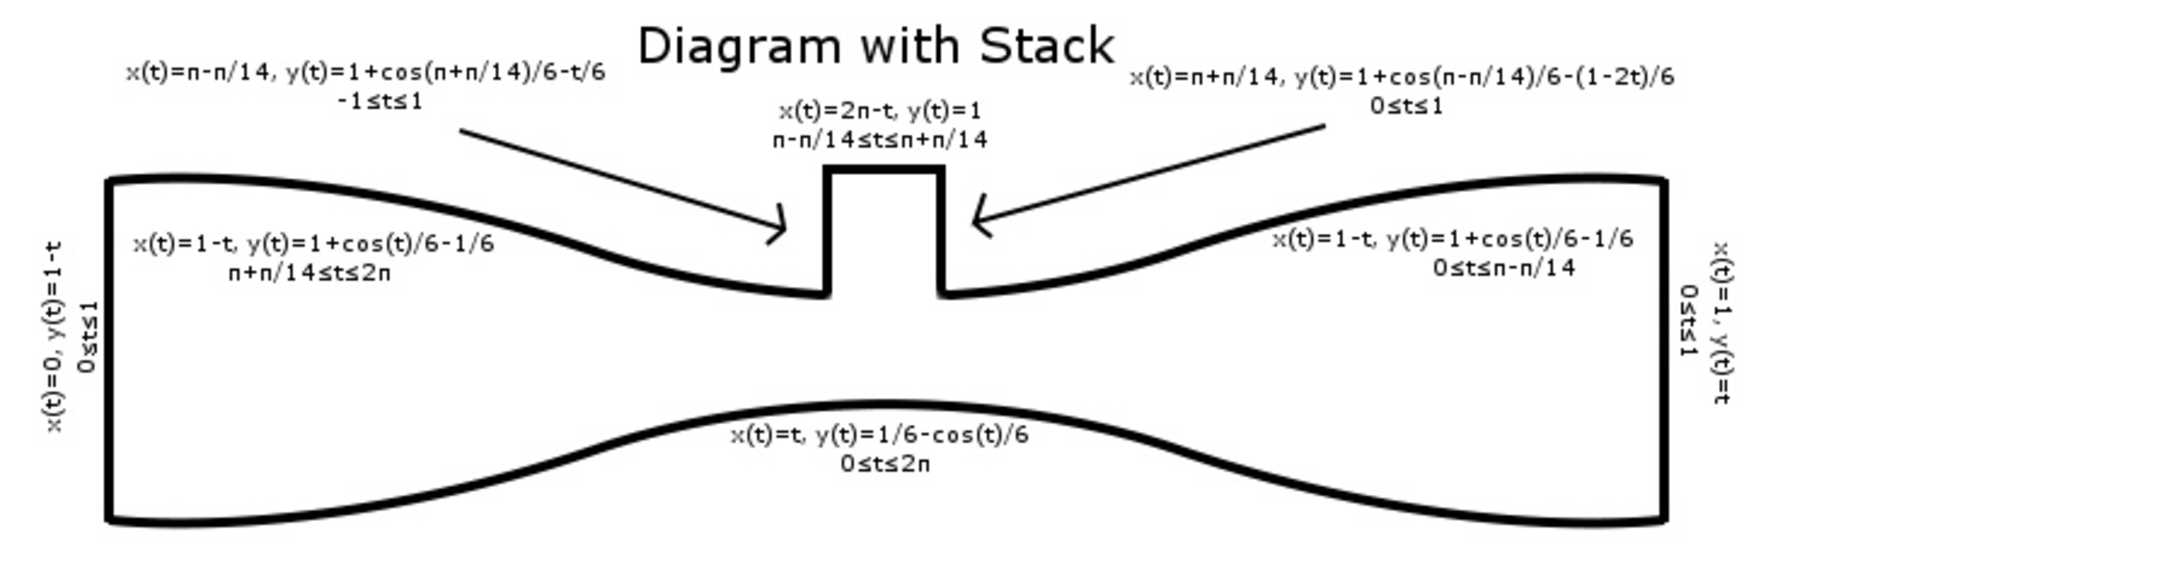
\includegraphics[width=1\textwidth,height=0.4\textwidth, viewport=0 0 900 300, clip]{diagram.pdf} 
\end{center}
\caption{\label{diagram}
Shown above is a diagram of the NSE-Voigt test problem}
\end{figure}


The inflow boundary condition was enforced to have a parabolic proflie with max velocity $u_{inlet}^{max}=1$.  At the two outlets, zero mean stress conditions were enforced, which were implemented as `do-nothing' conditions.  On the rest of the boundary, homogeneous Dirichlet conditions were enforced for the velocity.  We took the kinematic viscosity $\nu=0.001$, and started the flow from rest at T=0, and ran it out to T=4.

For this experiment, we used $(P_2,P_1^{disc})$ Scott-Vogelius elements, with a barycenter refined triangular mesh (a sufficient stability condition for Scott-Vogelius elements to be inf-sup stable).  These mixed finite elements have the attractive property that discrete velocity solutions are pointwise divergence, which is an important property for certain types of flows \cite{CELR10,linke09}.  In particular, for this test example, we also tested with $(P_2,P_1)$ Taylor-Hood elements and got very poor results without a very strong $L^2$ penalization of the size divergence with grad-div stabilization.  Hence, it seems Scott-Vogelius elements are a natural choice for this problem.

\begin{figure}[h!]
\begin{center}
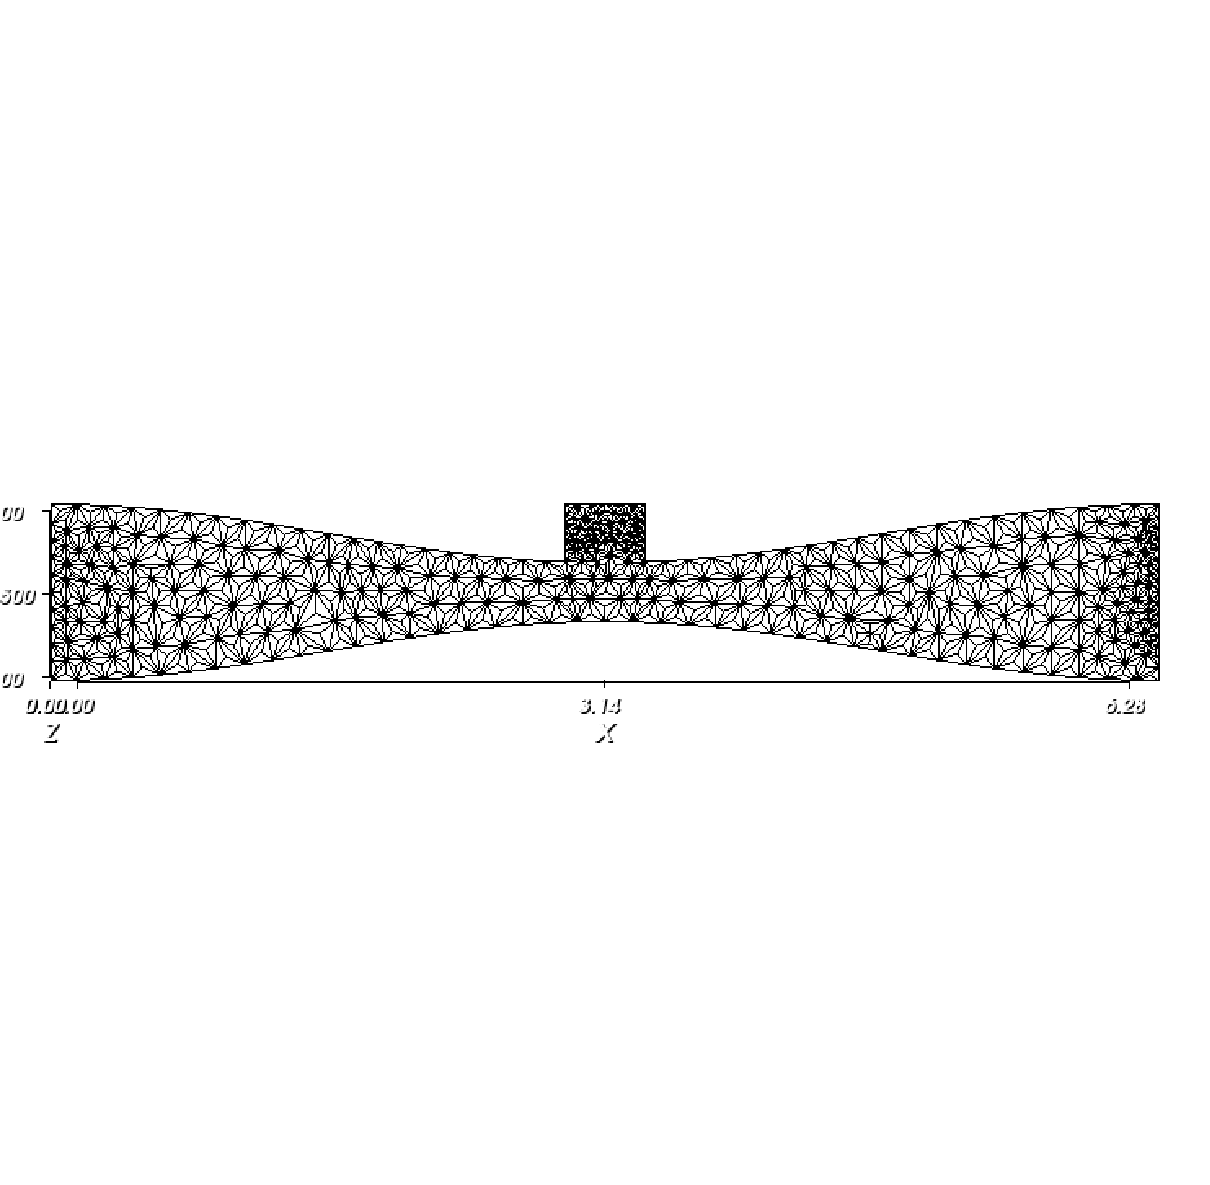
\includegraphics[width=.8\textwidth,height=0.16\textwidth, viewport=23 243 570 350, clip]{stackmeshbary.pdf} \\
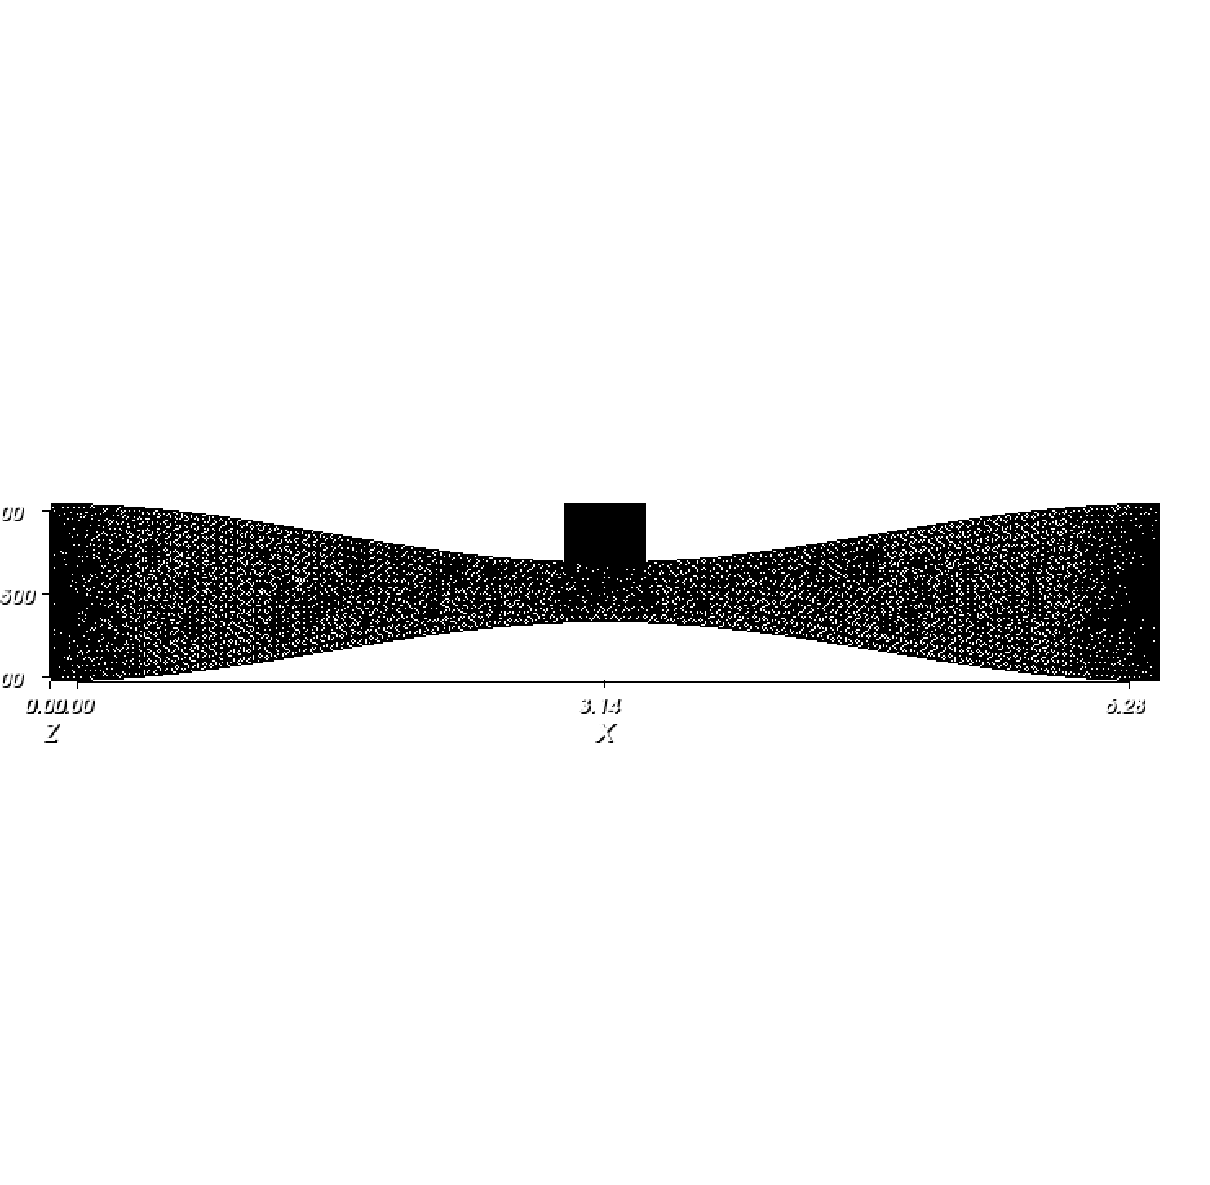
\includegraphics[width=.8\textwidth,height=0.16\textwidth, viewport=23 243 570 350, clip]{stackmeshbaryfine.pdf} 
\end{center}
\caption{\label{NSEmeshes}
Shown above are the meshes used in the numerical experiment for approximating NSE flows.}
\end{figure}

The meshes used in the computations are shown in Figure \ref{NSEmeshes}.  The coarse mesh provides 11,758 total degrees of freedom (dof), and the fine mesh provides 99,992 total dof.  We compute the NSE on the fine mesh (with $\alpha=0$) using \eqref{dnsev1}-\eqref{dnsev2} and timestep $\Delta t=0.01$, and believe this solution as the truth solution (based on numerous other computations on several other meshes and timesteps).  Plots of the velocity solution at T=1, 2, 3 and 4 are shown in Figure \ref{NSEfine}.  

\begin{figure}[h!]
\begin{center}
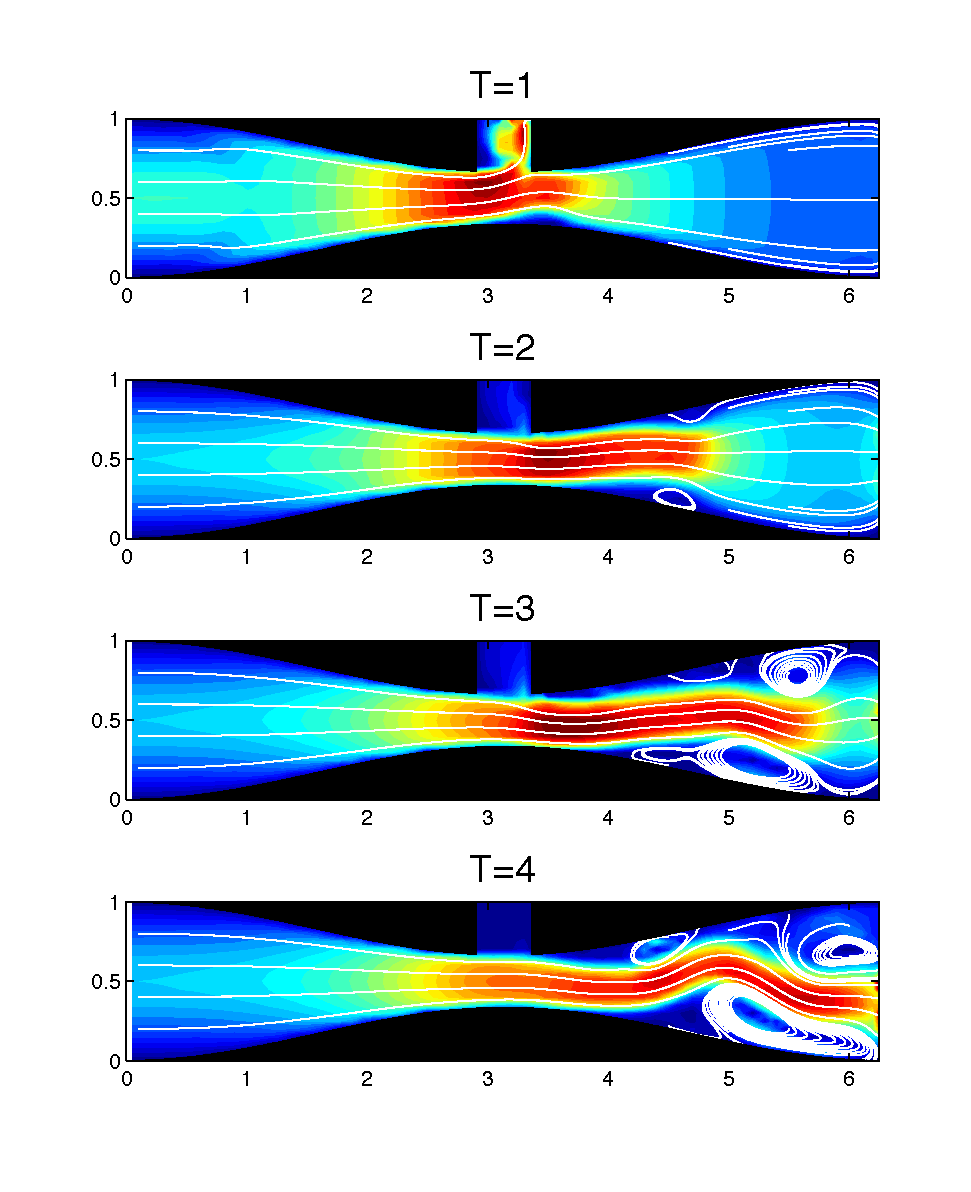
\includegraphics[width=.9\textwidth,height=0.8\textwidth, viewport=65 60 420 550, clip]{stackfine.pdf} 
\end{center}
\caption{\label{NSEfine}
Shown above is the fine mesh NSE solution at various times, displayed as velocity streamlines over speed contours.}
\end{figure}

The goal of the model we study is to produce good approximations to the solution, but using significantly less dof.  Hence we run \eqref{dnsev1}-\eqref{dnsev2} on the coarse mesh with parameter $\alpha=0.1 \approx h$.  For comparison, we also run the usual NSE ($\alpha=0$) on the same mesh.  Results at T=4 are shown in Figure \ref{NSEresults}.  We observe that on the coarse mesh, the usual NSE is underresolved, and significant numerical oscillations are present.  The NSE-Voigt plot, however, matches the overall flow pattern of the true solution well, and has significantly reduced oscillations compared to the NSE.


\begin{figure}[h!]
\begin{center}
NSE on coarse mesh at $T=4$ ($\alpha=0$)\\
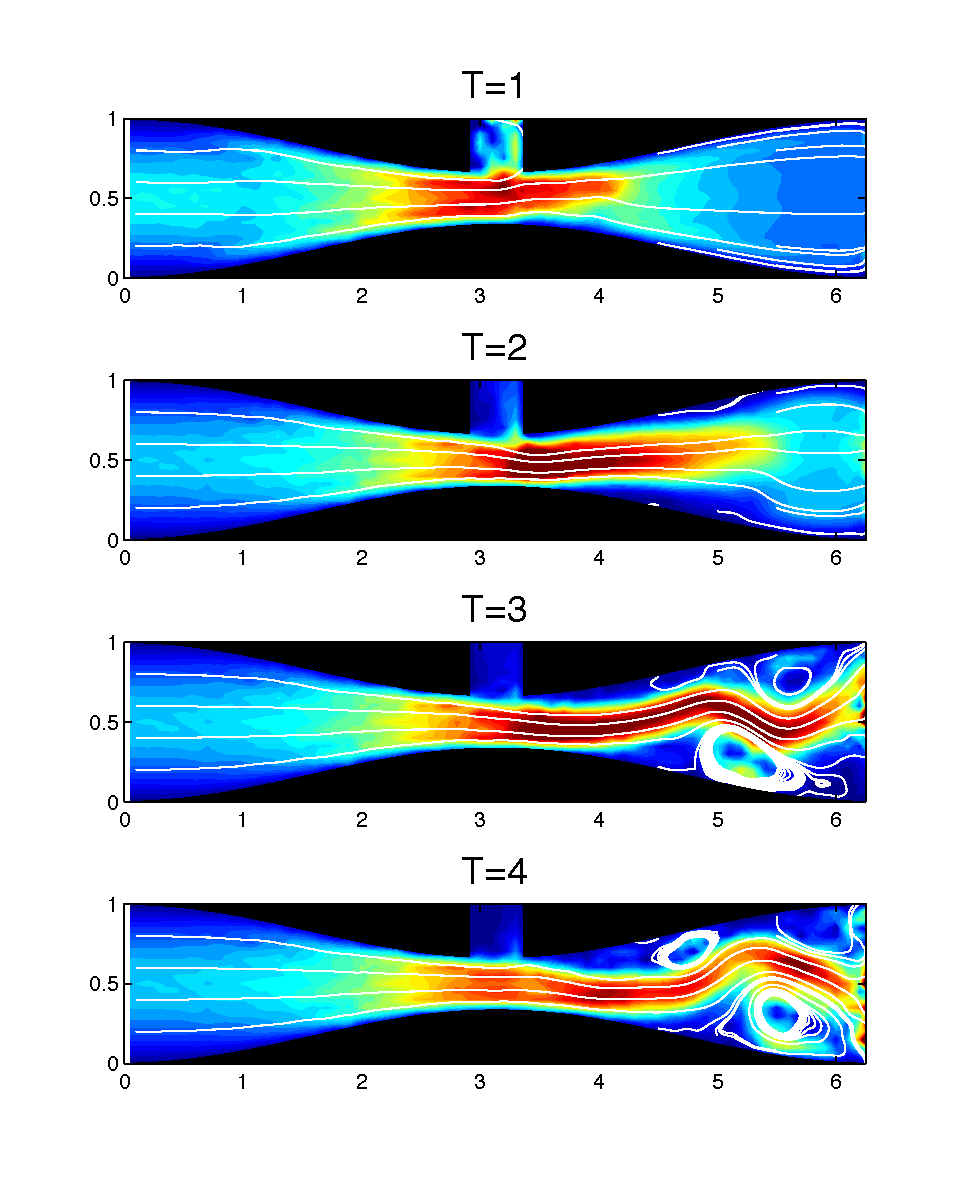
\includegraphics[width=.9\textwidth,height=0.15\textwidth, viewport=65 70 420 145, clip]{stackcoarse0.pdf} \vspace{.1in} \\
NSE-Voigt on coarse mesh at $T=4$ ($\alpha^2/\Delta t=1$)\\
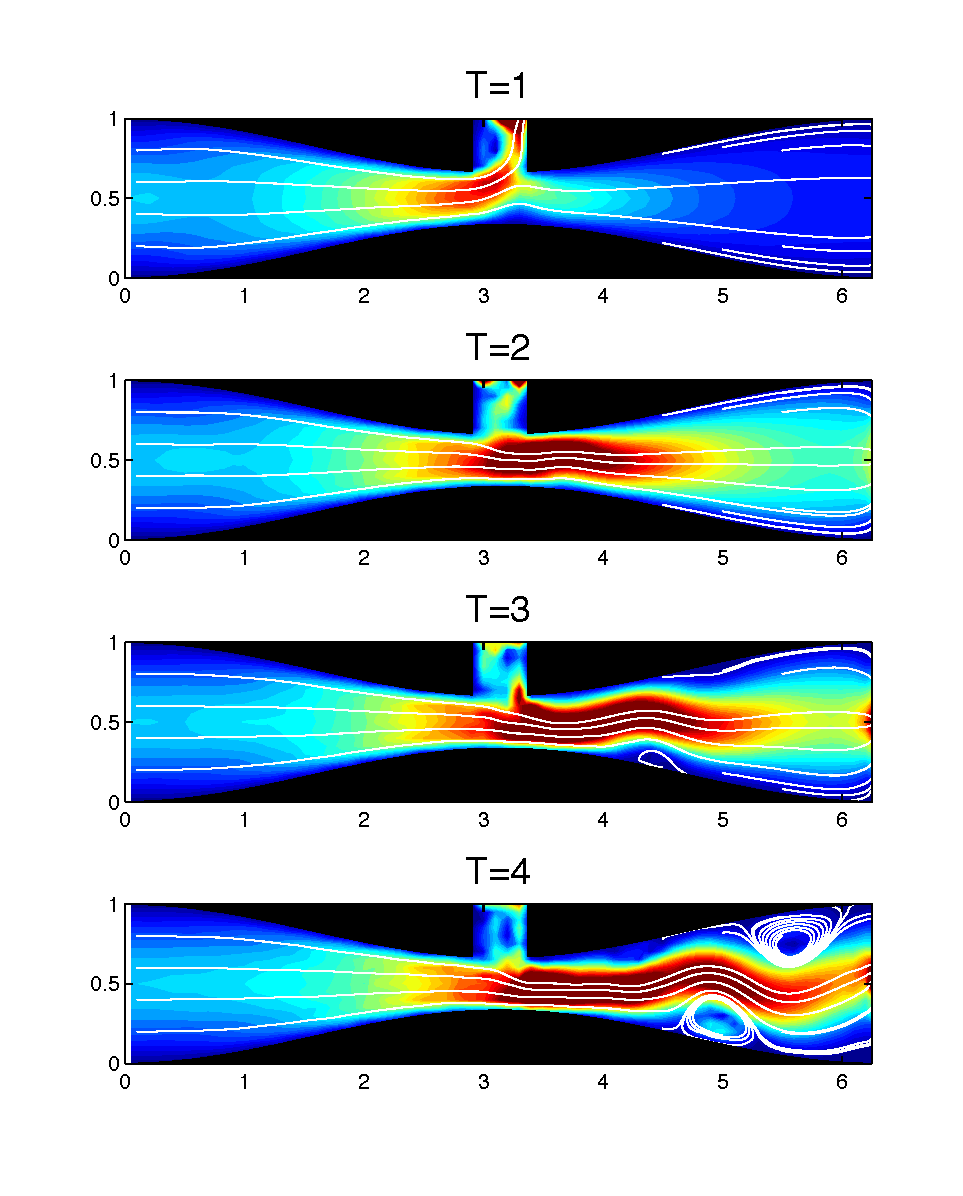
\includegraphics[width=.9\textwidth,height=0.15\textwidth, viewport=65 70 420 145, clip]{stackcoarse1.pdf} 
\caption{\label{NSEresults}
Shown above are the coarse mesh results at $T=4$ for NSE and NSE-Voigt, shown as velocity streamlines over speed contours.  Significant oscillations are present in the NSE solution, but are significantly reduced in the NSE-Voigt solution, which matches well the solution of the fine mesh NSE solution.}
\end{center}
\end{figure}




\section{A finite element algorithm for MHD-Voigt}

We now consider a finite element discretization of the Voigt regularization of evolution equations for incompressible magnetohydrodynamic (MHD) flows.  The following system of conservation laws governs the behavior of conducting, non-magnetic fluids, such as salt water, liquid metals, plasmas and strong electrolytes \cite{D01}.  It was
first developed by Ladyzhenskaya, has since been studied in \cite{GLP04,LP10,GT05,GT07,LW04}.  
\begin{eqnarray}
u_t + \nabla \cdot (uu^{T}) - Re^{-1}\Delta u + \frac{s}{2}\nabla(B\cdot B) - s\nabla \cdot{BB^T} + \nabla p & = & f, \label{mhd1}\\
\nabla \cdot u & = & 0, \label{mhd2} \\
B_t + Re_m^{-1}\nabla\times(\nabla \times B) + \nabla \times(B\times u)  & = & \nabla \times g, \label{mhd3} \\
\nabla \cdot B & = & 0. \label{mhd4}
\end{eqnarray}
Here, $u$ is velocity, $p$ is pressure, $f$ is body force, $\nabla \times g$ is a forcing
on the magnetic field $B$, $Re$ is the Reynolds number, $Re_m$ is the magnetic
Reynolds number, and $s$ is the coupling number.

The MHD-Voigt system is derived from \eqref{mhd1}-\eqref{mhd4} by adding a regularization term to each of the momentum and magnetic field equations, and takes the form
\begin{eqnarray}
u_t + \nabla \cdot (uu^{T}) - Re^{-1}\Delta u + \frac{s}{2}\nabla(B\cdot B) - s\nabla \cdot{BB^T} + \nabla p - \alpha_1^2\Delta u_t & = & f, \label{mhd1b}\\
\nabla \cdot u & = & 0, \label{mhd2b} \\
B_t + Re_m^{-1}\nabla\times(\nabla \times B) + \nabla \times(B\times u)  -\alpha_2^2 \Delta B_t & = & \nabla \times g, \label{mhd3b} \\
\nabla \cdot B & = & 0. \label{mhd4b}
\end{eqnarray}



We now proceed to derive a numerical scheme to approximate solutions to \eqref{mhd1b}-\eqref{mhd4b}, analyze its stability and convergence properties to solutions of \eqref{mhd1}-\eqref{mhd4}, and test it on benchmark problems.

We begin the derivation by expanding the curl operator in the \eqref{mhd3b} equation,
and using that $\nabla \cdot u=\nabla \cdot B=0$ to get
\begin{eqnarray}
u_t - Re^{-1}\Delta u  + u\cdot\nabla u  + \frac{s}{2}\nabla(B\cdot B) - s B \cdot \nabla B + \nabla p - \alpha_1^2 \Delta u_t & = & f, \label{mhd5} \\
\nabla \cdot u & = & 0, \label{mhd6} \\
B_t + Re_m^{-1}\nabla\times(\nabla \times B) + u\cdot\nabla B - B\cdot\nabla u - \alpha_2^2 \Delta B_t & = & \nabla \times g, \label{mhd7} \\
\nabla \cdot B & = & 0. \label{mhd8}
\end{eqnarray}
Denote by $P:=p+\frac{s}{2}\abs{B}^2$ a modified pressure, use a vector identity for the Laplacian, and define $\lambda:=Re_m \nabla\cdot B (=0)$, which will
act as a Lagrange multiplier corresponding to the solenoidal constraint of the magnetic field.  
When using mixed finite element methods to discretize the system, using the discrete dummy 
variable $\lambda$ in this way will allow for an explicit enforcement of a divergence free magnetic field.  We now have the system
\begin{eqnarray}
u_t  - Re^{-1}\Delta u + u\cdot\nabla u   - s B \cdot \nabla B + \nabla P - \alpha_1^2 \Delta u_t  & = & f, \\
\nabla \cdot u & = & 0, \\
B_t - Re_m^{-1}\Delta B  + u\cdot\nabla B - B\cdot\nabla u - \nabla \lambda - \alpha_2^2 \Delta B_t & = & \nabla \times g,\\
\nabla \cdot B & = & 0.
\end{eqnarray}
The numerical scheme is now derived with a Galerkin finite element spatial discretization and (four leg)
trapezoidal time discretization.  Denote $u_h^{n+\frac12}:=\frac12(u_h^n + u_h^{n+1})$.  We require the
discrete initial conditions be pointwise divergence free, that is, $u_h^0$ and $B_h^0$ must be in $V_h$.   For simplicity,
we will consider $u_h^0$ and $B_h^0$ to be defined to be the $H^1$ projections of solenoidal initial conditions $u_0$ and $B_0$ into $V_h$.  Then the resulting discrete problem
now reads: $\forall (v_h,\chi_h,q_h,r_h) \in (X_h,X_h,Q_h,Q_h)$, find $(u_h^{n+1},B_h^{n+1},P_h^{n+\frac12},\lambda_h^{n+\frac12})
\in (X_h,X_h,Q_h,Q_h)$ for $n=0,1,2,...,M=\frac{T}{\Delta t}$,
\begin{eqnarray}
\frac{1}{\Delta t}(u_{h}^{n+1}-u_{h}^{n},v_{h})
+ \frac{\alpha_1^2}{\Delta t}(\nabla (u_{h}^{n+1}- u_{h}^{n}),\nabla v_{h})
+ (u_{h}^{n+\frac{1}{2}} \cdot \nabla u_{h}^{n+\frac{1}{2}},v_{h})\nonumber\\
+Re^{-1}(\nabla u_{h}^{n+\frac{1}{2}},\nabla v_{h})
-s(B_{h}^{n+\frac{1}{2}} \cdot \nabla B_{h}^{n+\frac{1}{2}},v_{h})
-(P_{h}^{n+\frac{1}{2}},\nabla\cdot v_{h})
=(f(t^{n+\frac{1}{2}}),v_{h}), \label{Crank1}\\
(\nabla\cdot u_{h}^{n+1},q_{h}) = 0, \label{Crank2}\\
\frac{1}{\Delta t}(B_{h}^{n+1}-B_{h}^{n},\chi_{h})
+ \frac{\alpha_2^2}{\Delta t}(\nabla  (B_{h}^{n+1}- B_{h}^{n}),\nabla  \chi_{h})
+Re_{m}^{-1}(\nabla  B_{h}^{n+\frac{1}{2}},\nabla \chi_{h})\nonumber\\
-(B_{h}^{n+\frac{1}{2}} \cdot \nabla u_{h}^{n+\frac{1}{2}},\chi_{h})
+(u_{h}^{n+\frac{1}{2}}\cdot \nabla B_{h}^{n+\frac{1}{2}},\chi_{h})
+(\lambda_{h}^{n+\frac{1}{2}},\nabla\cdot\chi_{h})
=(\nabla\times g(t^{n+\frac{1}{2}}),\chi_{h}), \label{Crank3}\\
(\nabla\cdot B_{h}^{n+1},r_{h}) = 0. \label{Crank4}
\end{eqnarray}

\begin{remark}
A linearization of \eqref{Crank1}-\eqref{Crank4} can be derived by using linear extrapolation in the first component each of the 4 nonlinear terms via the substitution
\[
(u_h^{n+1/2} \cdot\nabla u_h^{n+1/2},v_h) \rightarrow 
\left((\frac{3}{2} u_h^{n} - \frac12 u_h^{n-1}) \cdot\nabla u_h^{n+1/2},v_h\right),
\]
and defining $u_h^{-1}:=u_h^0$ (and similarly for the other nonlinear terms).  The unconditional stability and convergence results that follow can be adapted to this linearized scheme with some minor, although technical, changes.
\end{remark}

\begin{remark}
We analyze the scheme in the case of homogeneous Dirichlet boundary conditions for both the velocity and magnetic field.  Extension to the periodic case is trivial, and extension to inhomogeneous Dirichlet boundaries can be done in the usual way.
\end{remark}

\subsection{Numerical analysis of the FE scheme for MHD-Voigt}

We prove here that the scheme is both unconditionally stable with respect to time-step, and optimally
convergent.  We begin with stability.

\begin{lem}
Solutions to the scheme \eqref{Crank1}-\eqref{Crank4} are stable for any $\Delta t>0$, provided $u_0 \in H^1(\Omega)$, 
$B_0\in H^1(\Omega)$, $f\in L^{2}(0,T;H^{-1}(\Omega))$ and $g\in L^{2}(0,T;L^{2}(\Omega))$, and satisfy
\begin{multline}
\norm{ u_{h}^{M}}^{2}+s\norm{B_{h}^{M}}^{2}+\alpha_1^2\norm{ \nabla u_{h}^{M} }+s\alpha_2^2 \norm{ \nabla B_{h}^{M} }
+\Delta t\sum_{n=0}^{M-1}{\left(Re^{-1}\norm{\nabla u_{h}^{n+\frac{1}{2}}}^{2}
+sRe_{m}^{-1}\norm{\nabla B_{h}^{n+\frac{1}{2}}}^{2}\right)} \\
\le
\norm{u_{h}^{0}}^{2}+s\norm{B_{h}^{0}}^{2} +\norm{\grad{u}_{h}^{0}}^{2}+s\norm{\grad{B}_{h}^{0}}^{2}
+\Delta t\sum_{n=0}^{M-1}{\left(
Re\norm{f(t^{n+\frac{1}{2}})}_{-1}^2 + sRe_m\norm{g(t^{n+\frac{1}{2}})}^2
\right)}\\ = C(Re,Re_m,f,g,u_0,B_0,s).
\end{multline}
\end{lem}
\begin{proof}
We begin this proof by setting $v_h=u_h^{n+1/2}$ and $\chi_h=B_h^{n+1/2}$ in \eqref{Crank1} and \eqref{Crank3} (which
are guaranteed to be in $V_h$ due to \eqref{Crank2} and \eqref{Crank4}), respectively, then adding the equations, multiplying through by $\Delta t$ and summing from $n=0$ to $M-1$.  This gives
\begin{multline}
\left(\frac12\left(\norm{ u_{h}^{M}}^{2}+\alpha_1^2\norm{\nabla u_{h}^{M}}\right)+\frac{s}{2}\left(\norm{B_{h}^{M}}^{2}+\alpha_2^2\norm{\nabla B_{h}^{M}}^{2}\right)\right)\\
+\Delta t\sum_{n=0}^{M-1}{\left(Re^{-1}\norm{\nabla u_{h}^{n+\frac{1}{2}}}^{2}
+sRe_{m}^{-1}\norm{\nabla B_{h}^{n+\frac{1}{2}}}^{2}\right)} \\
=
\left(\frac12\left(\norm{ u_{h}^{0}}^{2}+\alpha_1^2\norm{\nabla u_{h}^{0}}\right)+\frac{s}{2}\left(\norm{B_{h}^{0}}^{2}+\alpha_2^2\norm{\nabla B_{h}^{0}}^{2}\right)\right)\\
+\Delta t\sum_{n=0}^{M-1}{\left( (f(t^{n+\frac{1}{2}}),u_{h}^{n+\frac{1}{2}})
+s(\nabla\times g(t^{n+\frac{1}{2}}),B_{h}^{n+\frac{1}{2}})\right)} \label{stab0}
\end{multline}
The forcing terms can be majorized with Cauchy-Schwarz and Young's inequalities to get
\begin{eqnarray}
(f(t^{n+\frac{1}{2}}),u_{h}^{n+\frac{1}{2}})
& \le & 
\frac{Re}{2}\norm{f(t^{n+\frac{1}{2}})}_{-1}^2 + \frac{Re^{-1}}{2}\norm{\nabla u_h^{n+1/2}}^{2}, \label{stab1} \\
s(\nabla\times g(t^{n+\frac{1}{2}}),B_{h}^{n+\frac{1}{2}})
& \le &
\frac{sRe_m}{2}\norm{g(t^{n+\frac{1}{2}})}^2 + \frac{sRe^{-1}_{m}}{2}\norm{\nabla B_{h}^{n+\frac{1}{2}}}^2. \label{stab2}
\end{eqnarray}
Using \eqref{stab1} and \eqref{stab2} in \eqref{stab0} proves the lemma.
\end{proof}

We now prove convergence of the scheme.

\begin{theorem}
Assume $(u,p,B)$ solves \eqref{mhd1}-\eqref{mhd4} and satisfies the following regularity: $B_{t},u_{t}\in L^{\infty}(0,T;H^1(\Omega))$,
$B_{tt},u_{tt},\nabla B_{tt},\nabla u_{tt} \in L^{2}(0,T,L^2(\Omega))$,
$B_{ttt},u_{ttt}\in L^{2}(0,T;L^2(\Omega))$, and
$B,u\in L^{\infty}(0,T;H^{m}(\Omega))$, where $m=\max{(3,k)}$.  Then for $\Delta t$ small enough,
the solution  $(u_{h},p_{h},B_{h},\lambda_{h})$ to \eqref{Crank1}-\eqref{Crank4} converges to the true solution with rate
\[
\norm{ u-u_h}_{2,1} + \norm{B-B_h}_{2,1} = O(\Delta t^2 + h^k + \alpha_1^2 + \alpha_2^2).
\]
\end{theorem}

\begin{remark}
The convergence theorem shows that $\alpha_1,\alpha_2$ should be chosen to satisfy
\[
\alpha_1,\ \alpha_2 \leq C\max{ \{\Delta t,\ h^{k/2} \} }
\]
in order for the scheme to maintain optimal convergence.
\end{remark}



\begin{proof}
Throughout this proof, the constant C can depend on problem data and the true solution, can change its value at any step of the proof, but is independent of $h,\ \Delta t, \alpha_1,\ \alpha_2$.

Multiply the momentum and magnetic field equations  \eqref{mhd1}, \eqref{mhd3} at $t^{n+1/2}$ by $v_h\in V_h$ and $\chi_h \in V_h$, respectively, and
integrate over the domain.  Next, add $\frac{\alpha_1^2}{\Delta t}( \nabla u(t^{n+1}) - \nabla u(t^n),\nabla v_h)$ to both sides of the momentum equation, and $\frac{\alpha_2^2}{\Delta t}( \nabla B(t^{n+1}) - \nabla B(t^n),\nabla \chi_h)$ to both sides of the magnetic field equation.  Denoting $e^{k}_{u} = u^{k}_{h} - u^{k}$, $e^{k}_{B} = B^{k}_{h} - B^{k}$, we get
	\begin{multline}
	(u_{t}(t^{n+\frac{1}{2}}),v_{h}) + (u(t^{n+\frac{1}{2}})\cdot \grad{u}(t^{n+\frac{1}{2}}), v_{h}) + Re^{-1}(\grad{u}(t^{n+\frac{1}{2}}),\grad{v_{h}}) 
	 - s(B(t^{n+\frac{1}{2}})\cdot \grad{B}(t^{n+\frac{1}{2}}),v_{h})\\
	 +\alpha_1^2( \nabla u_{t}(t^{n+\frac{1}{2}}),\nabla v_h)
	+ \frac{\alpha_1^2}{\Delta t}( \nabla u(t^{n+1}) - \nabla u(t^n),\nabla v_h) \\
	 = (f(t^{n+\frac{1}{2}}),v_{h})  ) + \frac{\alpha_1^2}{\Delta t}( \nabla u(t^{n+1}) - \nabla u(t^n),\nabla v_h)
	\label{eq:3.34}
	\end{multline}
	\begin{multline}
	(B_{t}(t^{\nplushalf}),\chi_{h}) + Re^{-1}_{m}(\nabla B(t^{\nplushalf}),\grad{\chi_{h}}) - (B(t^{\nplushalf})\cdot \grad{u}(t^{\nplushalf}),\chi_{h}) \\
	 + (u(t^{\nplushalf})\cdot \grad{B}(t^{\nplushalf}),\chi_{h})+\alpha_2^2\nabla (B_{t}(t^{\nplushalf}),\nabla \chi_{h}) 
	 + \frac{\alpha_2^2}{\Delta t}( \nabla B(t^{n+1}) - \nabla B(t^n),\nabla \chi_h) \\
	 = (\nabla \times {g}(t^{\nplushalf}),\chi_{h}) + \frac{\alpha_2^2}{\Delta t}( \nabla B(t^{n+1}) - \nabla B(t^n),\nabla \chi_h).
	\label{eq:3.35}
	\end{multline}
	
	As usual, we will look to subtract the continuous formulation of the variational problem from the discrete formulation.  We start this process by introducing the following terms (\ref{eq:3.36})-(\ref{eq:3.40}), which replace the terms in the left-hand side of (\ref{eq:3.34}).  To simplify notation, we use $\pm$ to denote adding and subtracting the same term.
	\begin{equation}
	\begin{split}
	(u_{t}(t^{\nplushalf}),v_{h}) \pm \frac{1}{\Delta t}&(u(t^{n+1}) - u(t^{n}),v_{h}) = \frac{1}{\Delta t}(u(t^{n+1}) - u(t^{n}),v_{h}) \\
	& + (u_{t}(t^{\nplushalf}) - \{u(t^{n+1}) - u(t^{n})\}\Delta t^{-1},v_{h}).
	\end{split}
	\label{eq:3.36}
	\end{equation}

	\begin{equation}
	\begin{split}
	(u(t^{\nplushalf})\cdot \grad{u}(t^{\nplushalf}),v_{h}) & \pm (u^{\nplushalf}\cdot \grad{u}^{\nplushalf},v_{h}) = (u(t^{\nplushalf})\cdot \grad{(u(t^{\nplushalf}) - u^{\nplushalf})},v_{h}) \\
	& + ((u(t^{\nplushalf}) - u^{\nplushalf})\cdot \grad{u}^{\nplushalf},v_{h}) + (u^{\nplushalf} \cdot \grad{u}^{\nplushalf},v_{h}).
	\end{split}
	\label{eq:3.37}
	\end{equation}
	
	\begin{multline}
	Re^{-1}\left( (\grad{u}(t^{\nplushalf}),\grad{v_{h}}) \pm (\grad{u}^{\nplushalf},\grad{v_{h}}) \right)  \\ = Re^{-1}(\grad{(u(t^{\nplushalf}) - u^{\nplushalf})},\grad{v_{h}}) + Re^{-1}(\grad{u}^{\nplushalf},\grad{v_{h}})
	\label{eq:3.38}
	\end{multline}
		
	\begin{equation}
	\begin{split}
	-s(B(t^{\nplushalf})\cdot \grad{B}(t^{\nplushalf}),v_{h}) & \pm s(B^{\nplushalf}\cdot \grad{B}^{\nplushalf},v_{h}) = s(B^{\nplushalf}\cdot\grad{(B^{\nplushalf} - B(t^{\nplushalf}))},v_{h}) \\
	& + s((B^{\nplushalf} - B(t^{\nplushalf}))\cdot \grad{B}(t^{\nplushalf}),v_{h}) - s(B^{\nplushalf}\cdot \grad{B}^{\nplushalf},v_{h}).
	\end{split}
	\label{eq:3.40}
	\end{equation}
	
	\begin{equation}
	\begin{split}
	\alpha_1^2(\nabla u_{t}(t^{\nplushalf}),\nabla v_{h}) \pm \frac{\alpha_1^2}{\Delta t}&(\nabla (u(t^{n+1}) - u(t^{n})),\nabla v_{h}) = \frac{\alpha_1^2}{\Delta t}(\nabla (u(t^{n+1}) - u(t^{n})),\nabla v_{h}) \\
	& +\alpha_1^2(\nabla(u_{t}(t^{\nplushalf}) - \{u(t^{n+1}) - u(t^{n})\}\Delta t^{-1}),\nabla v_{h}).
	\end{split}
	\label{eq:3.62}
	\end{equation}

	Now we can directly subtract (\ref{eq:3.34}) from \eqref{Crank1},
	\begin{multline}
	\frac{1}{\Delta t}(e^{n+1}_{u} - e^{n}_{u},v_{h})  + Re^{-1}(\grad{e}^{\nplushalf}_{u},\grad{v_{h}})
	 + (u^{\nplushalf}_{h}\cdot\grad{e}^{\nplushalf}_{u},v_{h}) + (e^{\nplushalf}_{u}\cdot \grad{u}^{\nplushalf},v_{h}) \\
	  - s(B^{\nplushalf}_{h}\cdot \grad{e}^{\nplushalf}_{B},v_{h}) - s(e^{\nplushalf}_{B}\cdot\grad{B}^{\nplushalf},v_{h})+\frac{\alpha_1^2}{\Delta t}(\nabla (e_u^{n+1}-e_u^{n}),\nabla v_h) \\
	 = (u_{t}(t^{\nplushalf}) - \{u(t^{n+1}) - u(t^{n})\}\Delta t^{-1},v_{h}) + Re^{-1}(\grad{(u(t^{\nplushalf}) - u^{\nplushalf})},\grad{v_{h}}) \\
	 + (u(t^{\nplushalf})\cdot \grad{(u(t^{\nplushalf})-u^{\nplushalf})},v_{h}) + ((u(t^{\nplushalf}) - u^{\nplushalf})\cdot\grad{u}^{\nplushalf},v_{h})\\
	 	 + s((B^{\nplushalf}-B(t^{\nplushalf}))\cdot\grad{B}(t^{\nplushalf}),v_{h})
	 + s(B^{\nplushalf}\cdot \grad{(B^{\nplushalf} - B(t^{\nplushalf}))},v_{h})\\
%	+\alpha_1^2 (\nabla(u_{t}(t^{\nplushalf}) - \{u(t^{n+1}) - u(t^{n})\}\Delta t^{-1}),\nabla v_{h})
          + \alpha_1^2(\nabla u_{t}(t^{\nplushalf}),\nabla v_{h}) 
          - \alpha_1^2(\nabla(u_{t}(t^{\nplushalf}) - \{u(t^{n+1}) - u(t^{n})\}\Delta t^{-1}),\nabla v_{h})
	=: G_{1}(t,B,u,v_{h})
	\label{eq:3.41}
	\end{multline}
	
	Note that $G_{1}$ represents terms associated only with the true solution.
	Using the assumptions on the regularity of the solution, standard analysis (Taylor series, Cauchy-Schwarz and Young's inequalities, see e.g. \cite{Laytonbook}) provides
	\begin{eqnarray}
	| G_1(t,B,u,v_h) | &\le& C(\Delta t^2 \| v_h \|+\alpha_1^2(\Delta t^2+1)\norm{\grad{v}_h})\nonumber \\
	& \le & C\Delta t^4+C\norm{v_h}^2+\frac{Re^{-1}}{8}\norm{\grad{v}_h}^2+C\alpha_1^4\Delta t^4 + C\alpha_1^4.
	\label{g1bound}
	\end{eqnarray}
	
	Similarly for the magnetic field equation, we have
%	 to the derivation of (\ref{eq:3.41}) we introduce terms (\ref{eq:3.42})-(\ref{eq:3.43}) to the left hand side of (\ref{eq:3.35}) and then subtract from \eqref{Crank3}.
%	
%	\begin{equation}
%	\begin{split}
%	(B_{t}(t^{\nplushalf}),\chi_{h}) \pm \frac{1}{\Delta t}&(B(t^{n+1}) - B(t^{n}),\chi_{h}) = \frac{1}{\Delta t}(B(t^{n+1}) - B(t^{n}),\chi_{h}) \\
%	& + (B_{t}(t^{\nplushalf}) - \{B(t^{n+1}) - B(t^{n})\}\Delta t^{-1},\chi_{h}).
%	\end{split}
%	\label{eq:3.62}
%	\end{equation}
%
%	\begin{equation}
%	\begin{split}
%	-(B(t^{\nplushalf})\cdot \grad{u}(t^{\nplushalf}),\chi_{h}) \pm& (B^{\nplushalf}\cdot \grad{u}^{\nplushalf},\chi_{h}) = (B(t^{\nplushalf})\cdot\grad{(u^{\nplushalf} - u(t^{\nplushalf}))},\chi_{h}) \\
%	& + ((B^{\nplushalf} - B(t^{\nplushalf}))\cdot \grad{u}^{\nplushalf},\chi_{h})  - (B^{\nplushalf}\cdot\grad{u}^{\nplushalf},\chi_{h}).
%	\end{split}
%	\label{eq:3.42}
%	\end{equation}
%	
%	\begin{multline}
%	(u(t^{\nplushalf})\cdot\grad{(B(t^{\nplushalf}) - B^{\nplushalf})},\chi_{h}) \pm (u^{\nplushalf}\cdot\grad{B}^{\nplushalf},\chi_{h}) \\
%	 = (u(t^{\nplushalf})\cdot\grad{(B(t^{\nplushalf}) - B^{\nplushalf})},\chi_{h})
%	 + ((u(t^{\nplushalf}) - u^{\nplushalf})\cdot \grad{B}^{\nplushalf},\chi_{h}) \\
%	 + (u^{\nplushalf}\cdot\grad{B}^{\nplushalf},\chi_{h})
%	\label{eq:3.43}
%	\end{multline}
%
%	\begin{equation}
%	\begin{split}
%	\alpha_2^2(\nabla B_{t}(t^{\nplushalf}),\nabla \chi_{h}) \pm \frac{\alpha_2^2}{\Delta t}&(\nabla (B(t^{n+1}) - B(t^{n})),\nabla \chi_{h}) = \frac{\alpha_2^2}{\Delta t}(\nabla (B(t^{n+1}) - B(t^{n})),\nabla \chi_{h}) \\
%	& +\alpha_2^2 (\nabla (B_{t}(t^{\nplushalf}) - \{B(t^{n+1}) - B(t^{n})\}\Delta t^{-1}),\nabla \chi_{h}).
%	\end{split}
%	\label{eq:3.63}
%	\end{equation}
	\begin{equation}
	\begin{split}
	\frac{1}{\Delta t}(e^{n+1}_{B} - e^{n}_{B},\chi_{h}) & + Re^{-1}_{m}(\grad{e}^{\nplushalf}_{B},\grad{\chi}_{h}) - (B^{\nplushalf}_{h}\cdot \grad{e}^{\nplushalf}_{u},\chi_{h}) - (e^{\nplushalf}_{B}\cdot \grad{u}^{\nplushalf},\chi_{h})\\
& + (u^{\nplushalf}\cdot \grad{e}^{\nplushalf}_{B},\chi_{h}) + (e^{\nplushalf}_{u}\cdot \grad{B}^{\nplushalf},\chi_{h})+\frac{\alpha_2^2}{\Delta t}(\nabla (e^{n+1}_{B} - e^{n}_{B}),\nabla \chi_{h})  \\
	= (B_{t}(&t^{\nplushalf}) - \{B(t^{n+1}) - B(t^{n})\}\Delta t^{-1},\chi_{h}) \\
	& + Re^{-1}_{m}(\grad{(B(t^{\nplushalf}) - B^{\nplushalf})},\grad{\chi}_{h}) \\
	& + (B(t^{\nplushalf})\cdot\grad{(u^{\nplushalf} - u(t^{\nplushalf}))},\chi_{h}) + ((B^{\nplushalf} - B(t^{\nplushalf}))\cdot \grad{u}^{\nplushalf},\chi_{h}) \\
	& + (u(t^{\nplushalf})\cdot\grad{(B(t^{\nplushalf}) - B^{\nplushalf})},\chi_{h}) + ((u(t^{\nplushalf}) - u^{\nplushalf})\cdot\grad{B}^{\nplushalf},\chi_{h})\\
& + \alpha_2^2 (\nabla B_t(t^{n+\frac12}),\nabla \chi_h)- \alpha_2^2(\nabla(B_{t}(t^{\nplushalf}) - \{B(t^{n+1}) - B(t^{n})\}\Delta t^{-1}),\nabla \chi_{h}) \\
	=: G_{2}(&t,B,u,\chi_{h})
	\end{split}
	\label{eq:3.44}
	\end{equation}
	
	Similar to $G_1$, we bound $G_2$ by
	\begin{eqnarray}
	| G_2(t,B,u,v_h) |  & \le & C(\Delta t^2 \| \chi_h \|+\alpha_2^2(\Delta t^2+1)\norm{\grad{\chi}_h}) \nonumber \\
	& \le & C\Delta t^4 + C\norm{\chi}_h^2+\frac{Re^{-1}}{8}\norm{\grad{\chi}_h}^2+C\alpha_2^4\Delta t^4 +C\alpha_2^4. \label{g2bound}
	\end{eqnarray}


	Define $\phi^{n}_{h} = (u^{n}_{h} - U^{n})$ and $\eta^{n} = (u^{n} - U^{n}) \Rightarrow e^{n}_{u} = \phi^{n}_{h} - \eta^{n}_{u}$ and analogously $e^{n}_{B} = (B^{n}_{h} - \mathcal{B}^{n}) + (\mathcal{B}^{n} - B^{n}) = \psi^{n}_{h} - \eta^{n}_{B}$.  Where $U^{k} \in V_{h}$ and $\mathcal{B}^{k}\in V_{h}$.  Substituting into (\ref{eq:3.41}) and (\ref{eq:3.44}) results in:
	
	\begin{equation}
	\begin{split}
	\frac{1}{\Delta t}(\phi^{n+1}_{h} - \phi^{n}_{h},v_{h}) & + Re^{-1}(\grad{\phi}^{\nplushalf}_{h},\grad{v}_{h}) + (u^{\nplushalf}_{h}\cdot\grad{\phi}^{\nplushalf}_{h},v_{h}) + (\phi^{\nplushalf}_{h}\cdot\grad{u}^{\nplushalf},v_{h}) \\
	&  - s(B^{\nplushalf}_{h}\cdot\grad{\psi}^{\nplushalf}_{h},v_{h})
	 - s(\psi^{\nplushalf}_{h}\cdot\grad{B}^{\nplushalf},v_{h}) +\frac{\alpha_1^2}{\Delta t}(\nabla (\phi^{n+1}_{h} - \phi^{n}_{h}),\grad{v}_{h})\\
	=\frac{1}{\Delta t}(\eta^{n+1}_{u}& - \eta^{n}_{u},v_{h}) + Re^{-1}(\grad{\eta}^{\nplushalf}_{u},\grad{v}_{h}) + (u^{\nplushalf}_{h}\cdot\grad{\eta}^{\nplushalf}_{u},v_{h}) \\
	& + (\eta^{\nplushalf}_{u}\cdot\grad{u}^{\nplushalf},v_{h}) - s(B^{\nplushalf}_{h}\cdot \eta^{\nplushalf}_{B},v_{h}) - s(B^{\nplushalf}_{h}\cdot\grad{\eta}^{\nplushalf}_{B},v_{h}) \\
	& - s(\eta^{\nplushalf}_{B}\cdot \grad{B}^{\nplushalf},v_{h})+\frac{\alpha_1^2}{\Delta t}(\nabla (\eta^{n+1}_{u} - \eta^{n}_{u}),\grad{v}_{h})
	+ G_{1}(t,u,B,v_{h})
	\end{split}
	\label{eq:3.45}
	\end{equation}
	
	\begin{equation}
	\begin{split}
	\frac{1}{\Delta t}(\psi^{n+1}_{h} - \psi^{n}_{h},\chi_{h}) & + Re^{-1}_{m}(\grad{\psi}^{n+1}_{h},\grad{\chi}_{h}) - (B^{\nplushalf}_{h}\cdot\grad{\phi}^{\nplushalf}_{h},\chi_{h}) - (\psi^{\nplushalf}_{h}\cdot\grad{u}^{\nplushalf},\chi_{h}) \\
	& + (u^{\nplushalf}\cdot\grad{\psi}^{\nplushalf}_{h},\chi_{h}) + (\phi^{\nplushalf}_{h}\cdot\grad{B}^{\nplushalf},\chi_{h})+\frac{\alpha_2^2}{\Delta t}(\nabla (\psi^{n+1}_{h} - \psi^{n}_{h}),\grad{\chi}_{h}) \\
	= \frac{1}{\Delta t}(\eta^{n+1}_{B} & - \eta^{n}_{B},\chi_{h}) + Re^{-1}_{m}(\grad{\eta}^{\nplushalf}_{B}, \grad{\chi}_{h}) - (B^{\nplushalf}_{h}\cdot \grad{\eta}^{\nplushalf}_{u},\chi_{h}) \\
	& - (\eta^{\nplushalf}_{B}\cdot\grad{u}^{\nplushalf},\chi_{h}) + (u^{\nplushalf}\cdot\grad{\eta}^{\nplushalf}_{B},\chi_{h}) + (\eta^{\nplushalf}_{u}\cdot\grad{B}^{\nplushalf},\chi_{h}) \\&+\frac{\alpha_2^2}{\Delta t}(\nabla (\eta^{n+1}_{b} - \eta^{n}_{b}),\grad{\chi}_{h}) 
	 + G_{2}(t,u,B,\chi_{h})
	\end{split}
	\label{eq:3.46}
	\end{equation}
	
	Taking $\chi_{h} = \psi^{\nplushalf}_{h}$ and $v_{h} = \phi^{\nplushalf}_{h}$ in (\ref{eq:3.45}) and (\ref{eq:3.46}), then simplifying yields the equations
	
	\begin{equation}
	\begin{split}
	\frac{1}{2\Delta t}(\norm{\phi^{n+1}_{h}}^{2} - \norm{\phi^{n}_{h}}^{2}) & + Re^{-1}\norm{\nabla \phi^{\nplushalf}_{h}}^{2} + (\phi^{\nplushalf}_{h}\cdot\grad{u}^{\nplushalf},\phi^{\nplushalf}_{h}) 
	 - s(B^{\nplushalf}_{h}\cdot\grad{\psi^{\nplushalf}_{h}},\phi^{\nplushalf}_{h}) \\&- s(\psi^{\nplushalf}_{h}\cdot\grad{B}^{\nplushalf},\phi^{\nplushalf}_{h}) +\frac{\alpha_1^2}{2\Delta t}(\norm{\grad{\phi}^{n+1}_{h}}^{2} - \norm{\grad{\phi}^{n}_{h}}^{2}) \\
	= \frac{1}{\Delta t}(\eta^{n+1}_{u} & - \eta^{n}_{u},\phi^{\nplushalf}_{h}) + Re^{-1}(\grad{\eta}^{\nplushalf}_{u},\grad{\phi^{\nplushalf}_{h}}) + (u^{\nplushalf}_{h}\cdot\grad{\eta}^{\nplushalf}_{u},\phi^{\nplushalf}_{h}) \\
	& + (\eta^{\nplushalf}_{u}\cdot\grad{u}^{\nplushalf},\phi^{\nplushalf}_{h}) - s(B^{\nplushalf}_{h}\cdot \grad{\eta}^{\nplushalf}_{B},\phi^{\nplushalf}_{h}) - s(\eta^{\nplushalf}_{B}\cdot \grad{B}^{\nplushalf},\phi^{\nplushalf}_{h}) \\& + \frac{\alpha_1^2}{\Delta t}(\grad{\eta}^{n+1}_{u} - \grad{\eta}^{n}_{u},\grad{\phi}^{\nplushalf}_{h})+ G_{1}(t,u,B,\phi^{\nplushalf}_{h})
	\end{split}
	\label{eq:3.47}
	\end{equation}
	and 
	\begin{multline}
	\frac{1}{2\Delta t}\left(\norm{\psi^{\nplushalf}_{h}}^{2} - \norm{\psi^{\nplushalf}_{h}}^{2}\right)  + Re^{-1}_{m}\norm{\grad{\psi^{\nplushalf}_{h}}}^{2} - (B^{\nplushalf}_{h} \cdot \grad{\phi^{\nplushalf}_{h}},\psi^{\nplushalf}_{h}) - (\psi^{\nplushalf}_{h}\cdot\grad{u}^{\nplushalf},\psi^{\nplushalf}_{h}) \\
+ (\phi^{\nplushalf}_{h}\cdot \grad{B}^{\nplushalf},\psi^{\nplushalf}_{h}) + \frac{\alpha_2^2}{2\Delta t}\left(\norm{\grad{\psi}^{\nplushalf}_{h}}^{2} - \norm{\grad{\psi}^{\nplushalf}_{h}}^{2}\right)\\
= \frac{1}{\Delta t}(\eta^{n+1}_{B}  - \eta^{n}_{B},\psi^{\nplushalf}_{h})
	 + Re^{-1}_{m}(\grad{\eta}^{\nplushalf}_{B},\grad{\psi^{\nplushalf}_{h}}) - (B^{\nplushalf}_{h}\cdot\grad{\eta}^{\nplushalf}_{u},\psi^{\nplushalf}_{h}) \\
	- (\eta^{\nplushalf}_{B}\cdot\grad{u}^{\nplushalf},\psi^{\nplushalf}_{h}) + (u^{\nplushalf}\cdot\grad{\eta}^{\nplushalf}_{B},\psi^{\nplushalf}_{h})
	 + (\eta^{\nplushalf}_{u}\cdot\grad{B}^{\nplushalf},\psi^{\nplushalf}_{h}) \\
	+  \frac{\alpha_2^2}{\Delta t}(\grad{\eta}_B^{n+1}-\grad{\eta}_B^{n},\grad{\psi}_h^\nplushalf)+ G_{2}(t,u,B,\psi^{\nplushalf}_{h})
	\label{eq:3.48}
	\end{multline}
	
	Using the inequalities,
	\begin{equation}
	\frac{1}{\Delta t}(\eta^{n+1}_{u} - \eta^{n}_{u},\phi^{\nplushalf}_{h}) \leq \frac{1}{2\Delta t}\int^{t^{n+1}}_{t^{n}} \norm{\partial(\eta_{u})}^{2}\, dt + \frac{1}{2}\norm{\phi^{\nplushalf}_{h}}^{2},
	\label{eq:3.49}
	\end{equation}

	\begin{equation}
	\frac{\alpha_1^2}{\Delta t}(\grad{\eta}^{n+1}_{u} - \grad{\eta}^{n}_{u},\grad{\phi}^{\nplushalf}_{h}) \leq \frac{\alpha_1^2}{2\Delta t}\int^{t^{n+1}}_{t^{n}} \norm{\partial(\grad{\eta}_{u})}^{2}\, dt + \frac{\alpha_1^2}{2}\norm{\grad{\phi}^{\nplushalf}_{h}}^{2},
	\label{eq:3.49}
	\end{equation}
	
	\noindent along with H\"{o}lder's Inequality and \eqref{g1bound},
	\begin{multline}
	\frac{1}{2\Delta t}(\norm{\phi^{n+1}_{h}}^{2} - \norm{\phi^{n}_{h}}^{2})  + \frac{Re^{-1}}{2}\norm{\nabla \phi^{\nplushalf}_{h}}^{2}+\frac{\alpha_1^2}{2\Delta t}(\norm{\grad{\phi}^{n+1}_{h}}^{2} - \norm{\grad{\phi}^{n}_{h}}^{2}) \\
	\leq \frac{1}{2\Delta t}\int^{t^{n+1}}_{t^{n}} (\norm{\partial_{t}(\eta_{u})}^{2}+\alpha_1^2\norm{\grad{\partial_{t}(\eta_{u})}}^{2}\, )dt + \frac{1}{2}\norm{\phi^{\nplushalf}_{h}}^{2}+\frac{\alpha_1^2}{2}\norm{\grad{\phi}^{\nplushalf}_{h}}^{2} + \left(\frac{Re^{-1}}{2}\right)\norm{\eta^{\nplushalf}_{u}}^{2} \\
	+ \norm{\nabla u^{\nplushalf}}_{\infty}\norm{\phi_h^{\nplushalf}}^2
	+ s(B_h^{\nplushalf}\cdot\nabla \psi_h^{\nplushalf},\phi_h^{\nplushalf})
	+ s\norm{\nabla B^{\nplushalf}}_{\infty}\norm{\psi_h^{\nplushalf}}\norm{\phi_h^{\nplushalf}} \\
	+ C\norm{\nabla u_h^{\nplushalf}}\norm{\nabla \eta_u^{\nplushalf}}\norm{\nabla \phi_h^{\nplushalf}}
	+ \norm{\nabla u^{\nplushalf}}_{\infty}\norm{\eta_u^{\nplushalf}}\norm{\phi_h^{\nplushalf}}
         + Cs\norm{\nabla B_h^{\nplushalf}}\norm{\nabla \eta_B^{\nplushalf}}\norm{\nabla \phi_h^{\nplushalf}} \\
         + s\norm{\nabla B^{\nplushalf}}_{\infty}\norm{\eta_B^{\nplushalf}}\norm{\phi_h^{\nplushalf}}
         +C\left(\Delta t^4 + \norm{\phi^{\nplushalf}} + \alpha_1^4 + \alpha_1^4 \Delta t^4\right)
	\label{eq:3.50}
	\end{multline}
	
This reduces, with Cauchy-Schwarz and Young's inequalities and the assumption of the regularity of the solution, to
	\begin{multline}
	\frac{1}{2\Delta t}(\norm{\phi^{n+1}_{h}}^{2} - \norm{\phi^{n}_{h}}^{2})  + \frac{Re^{-1}}{8}\norm{\nabla \phi^{\nplushalf}_{h}}^{2}+\frac{\alpha_1^2}{2\Delta t}(\norm{\grad{\phi}^{n+1}_{h}}^{2} - \norm{\grad{\phi}^{n}_{h}}^{2}) \\
	\leq \frac{1}{2\Delta t}\int^{t^{n+1}}_{t^{n}} (\norm{\partial_{t}(\eta_{u})}^{2}+\alpha_1^2\norm{\grad{\partial_{t}(\eta_{u})}}^{2}\, )dt  +\frac{\alpha_1^2}{2}\norm{\grad{\phi_h^{\nplushalf}}}^2+ \left(\frac{Re^{-1}}{2}\right)\norm{\grad{\eta}^{\nplushalf}_{u}}^{2} \\
	+ C(\norm{\phi_h^{\nplushalf}}^2 + \norm{\psi_h^{\nplushalf}}^2 + \Delta t^4+\Delta t^4 \alpha_1^4 + \alpha_1^4\Delta t^4
	+ \norm{\eta_u^{\nplushalf}}^2 + \norm{\nabla u_h^{\nplushalf}}^2\norm{\nabla \eta_u^{\nplushalf}}^2\\
	+ s^2\norm{\nabla B_h^{\nplushalf}}^2\norm{\nabla \eta_B^{\nplushalf}}^2 
	+ s^2 \norm{\eta_B^{\nplushalf}}^2)	
	+ s(B_h^{\nplushalf}\cdot\nabla \psi_h^{\nplushalf},\phi_h^{\nplushalf})
	\label{eq:3.56}
	\end{multline}
	We now step back from (\ref{eq:3.56}) and return to (\ref{eq:3.48}), which can be majorized in a similar way as the momentum system, as
	\begin{multline}
	\frac{1}{2\Delta t}(\norm{\psi^{n+1}_{h}}^{2} - \norm{\psi^{n}_{h}}^{2}) + \frac{Re^{-1}_{m}}{2}\norm{\grad{\psi^{n+1/2}_{h}}}^{2}+\frac{\alpha_2^2}{2\Delta t}(\norm{\grad{\psi}^{n+1}_{h}}^{2} - \norm{\grad{\psi}^{n}_{h}}^{2})\\
	 	\leq \frac{1}{2\Delta t} \int^{t^{n+1}}_{t^{n}}  (\norm{\partial_{t}(\eta_{B})}^{2}+\alpha_2^2\norm{\grad{\partial_{t}(\eta_{B})}}^{2}\, )dt 
	 + \frac{1}{2}\norm{\psi^{\nplushalf}_{h}}^{2} + \frac{\alpha_2^2}{2}\norm{\grad{\psi}^{\nplushalf}_{h}}^{2}+ Re^{-1}_{m}\norm{\grad{\eta^{\nplushalf}_{B}}}^{2}\\
	 + (B^{\nplushalf}_{h} \cdot \grad{\phi^{\nplushalf}_{h}}, \psi^{\nplushalf}_{h})
	 + \norm{\nabla B^{\nplushalf}}_{\infty}\norm{\phi_h^{\nplushalf}}\norm{\psi_h^{\nplushalf}}
	 + \norm{\nabla u^{\nplushalf}}_{\infty}\norm{\psi_h^{\nplushalf}}^2\\
	  + C\norm{\nabla B_h^{\nplushalf}}\norm{\nabla \eta_u^{\nplushalf}}\norm{\nabla \psi_h^{\nplushalf}}
	 + C\norm{\nabla u^{\nplushalf}}_{\infty}\norm{\nabla \eta_B^{\nplushalf}}\norm{\psi_h^{\nplushalf}}\\
	 + \norm{\nabla B^{\nplushalf}}_{\infty}\norm{\eta_u^{\nplushalf}}\norm{\psi_h^{\nplushalf}}
%	+C\left(\Delta t^2 \norm{\psi_h^{\nplushalf}}+\alpha_2^2\Delta t^2\norm{\grad{\psi}_h^{\nplushalf}}\right)
	         +C\left(\Delta t^4 + \norm{\psi^{\nplushalf}} + \alpha_2^4 + \alpha_2^4 \Delta t^4\right)
	 \end{multline}
	
	 Under the regularity assumptions, Cauchy-Schwarz and Young's inequalities, this can be reduced to
	\begin{multline}
	\frac{1}{2\Delta t}(\norm{\psi^{n+1}_{h}}^{2} - \norm{\psi^{n}_{h}}^{2}) + \frac{Re^{-1}_{m}}{8}\norm{\grad{\psi^{n+1}_{h}}}^{2}+\frac{\alpha_2^2}{2\Delta t}(\norm{\grad{\psi}^{n+1}_{h}}^{2} - \norm{\grad{\psi}^{n}_{h}}^{2})\\
	 \leq \frac{1}{2\Delta t} \int^{t^{n+1}}_{t^{n}} (\norm{\partial_{t}(\eta_{B})}^{2}+\alpha_2^2\norm{\partial_{t}(\grad{\eta}_{B})}^{2})\, dt
	 + \frac{\alpha_2^2}{2}\norm{\grad{\psi_h^{\nplushalf}}}^2 \\+ Re^{-1}_{m}\norm{\grad{\eta^{\nplushalf}_{B}}}^{2}
	 + C( \norm{\psi_h^{\nplushalf}}^2 + \Delta t^4 +\Delta t^4 \alpha_2^2+ \alpha_2^4+ \norm{\phi_h^{\nplushalf}}^2
	 + \norm{\nabla \eta_B^{\nplushalf}}^2
	 + \norm{\eta_u^{\nplushalf}}^2 \\
	 + Re \norm{\nabla B_h^{\nplushalf}}^2\norm{\nabla \eta_u^{\nplushalf}}^2)
	 + (B^{\nplushalf}_{h} \cdot \grad{\phi^{\nplushalf}_{h}}, \psi^{\nplushalf}_{h}).
	 \label{eq:3.58}
	 \end{multline}
	 Multiplying \eqref{eq:3.58} by $s$ and adding it to \eqref{eq:3.56}, and using that
         \[
         (B^{\nplushalf}_{h} \cdot \grad{\phi^{\nplushalf}_{h}}, \psi^{\nplushalf}_{h})
         =
         -(B^{\nplushalf}_{h} \cdot \grad{\psi^{\nplushalf}_{h}}, \phi^{\nplushalf}_{h}),
         \]
         along with Poincare's inequality and reducing, we get
         	\begin{multline}
	\frac{1}{2\Delta t}(\norm{\phi^{n+1}_{h}}^{2} - \norm{\phi^{n}_{h}}^{2})
	 + \frac{s}{2\Delta t}(\norm{\psi^{n+1}_{h}}^{2} - \norm{\psi^{n}_{h}}^{2})
          + \frac{Re^{-1}}{8}\norm{\nabla \phi^{\nplushalf}_{h}}^{2}
	 + \frac{sRe^{-1}_{m}}{8}\norm{\grad{\psi^{n+1/2}_{h}}}^{2} \\+\frac{\alpha_1^2}{2\Delta t}(\norm{\grad{\phi}^{n+1}_{h}}^{2} - \norm{\grad{\phi}^{n}_{h}}^{2})+\frac{\alpha_2^2}{2\Delta t}(\norm{\grad{\psi}^{n+1}_{h}}^{2} - \norm{\grad{\psi}^{n}_{h}}^{2})\\
	\leq
	\frac{1}{2\Delta t}\int^{t^{n+1}}_{t^{n}} \left(\norm{\partial_{t}(\eta_{u})}^{2}+\alpha_1^2\norm{\partial_{t}(\grad{\eta}_{u})}^{2}\right)\, dt
	+ \frac{s}{2\Delta t} \int^{t^{n+1}}_{t^{n}}\left( \norm{\partial_{t}(\eta_{B})}^{2}+\alpha_2^2\norm{\partial_{t}(\grad{\eta}_{B})}^{2}\right)\, dt\\
	+ \frac{\alpha_1^2}{2}\norm{\grad{\phi_h^{\nplushalf}}}^2
	+\frac{s\alpha_2^2}{2}\norm{\grad{\psi_h^{\nplushalf}}}^2
	+ \left(\frac{Re^{-1}}{2}\right)\norm{\grad{\eta}^{\nplushalf}_{u}}^{2}
	+ \left(\frac{sRe^{-1}_{m}}{2}\right)\norm{\grad{\eta^{\nplushalf}_{B}}}^{2}\\
	+C(s)(\norm{\phi_h^{\nplushalf}}^2 + \norm{\psi_h^{\nplushalf}}^2 
	+ \Delta t^4+\Delta t^4 \alpha_1^2 +\Delta t^4 \alpha_2^2 + \alpha_1^4 + \alpha_2^4
	+ \norm{\eta_u^{\nplushalf}}^2 + \norm{\nabla u_h^{\nplushalf}}^2\norm{\nabla \eta_u^{\nplushalf}}^2\\
	+ \norm{\nabla B_h^{\nplushalf}}^2\norm{\nabla \eta_B^{\nplushalf}}^2 
	+  \norm{\nabla \eta_B^{\nplushalf}}^2
	+ Re \norm{\nabla B_h^{\nplushalf}}^2\norm{\nabla \eta_u^{\nplushalf}}^2
	)
	\label{eq:3.59}
	\end{multline}

         Multiplying by $2\Delta t$ and summing over timesteps now gives
         	\begin{multline}
	\norm{\phi^{M}_{h}}^{2}  + s\norm{\psi^{M}_{h}}^{2}
          + \sum_{n=0}^{M-1} \left( Re^{-1}\norm{\nabla \phi^{\nplushalf}_{h}}^{2} +
	 	 sRe^{-1}_{m}\norm{\grad{\psi^{n+\frac12}_{h}}}^{2} \right)+\alpha_1^2\norm{\grad{\phi_h^M}}^2+s\alpha_2^2\norm{\grad{\psi_h^M}}^2 \\
	\leq
	C\int^{T}_{0} \left( \norm{\partial_{t}(\eta_{u})}^{2} + \norm{\partial_{t}(\grad{\eta}_{u})}^{2} + s \norm{\partial_{t}(\eta_{B})}^{2} +s \norm{\partial_{t}(\grad{\eta}_{B})}^{2}\right) \, dt\\
	+ CT(\Delta t^4(1+\alpha_1^4+\alpha_2^4) + \alpha_1^4 + \alpha_2^4 ) 
	+ C\Delta t \sum_{n=0}^{M-1}( \norm{\nabla \eta^{\nplushalf}_{u}}^{2}
		+ \norm{\grad{\eta^{\nplushalf}_{B}}}^{2} 
		+ \norm{\nabla u_h^{\nplushalf}}^2\norm{\nabla \eta_u^{\nplushalf}}^2\\
		+ \norm{\nabla B_h^{\nplushalf}}^2\norm{\nabla \eta_B^{\nplushalf}}^2
		+ \norm{\nabla B_h^{\nplushalf}}^2\norm{\nabla \eta_u^{\nplushalf}}^2
	) \\
	+ \Delta t C\sum_{n=0}^{M-1}\left(\norm{\phi_h^{n+1}}^2+\alpha_1^2\norm{\grad{\phi}_h^{n+1}}^2 + s\norm{\psi_h^{n+1}}^2 + s\alpha_2^2\norm{\grad{\psi}_h^{n+1}}^2\right )\\
	\label{eq:3.60}
	\end{multline}
         Next we use approximation properties of the spaces and the stability estimate, which reduces \eqref{eq:3.60} to
         	\begin{multline}
	\norm{\phi^{M}_{h}}^{2}  + s\norm{\psi^{M}_{h}}^{2}+\alpha_1^2\norm{\grad{\phi_h^M}}^2
	+s\alpha_2^2\norm{\grad{\psi_h^M}}^2 \\
          +\Delta t \sum_{n=0}^{M-1} \left( Re^{-1}\norm{\nabla \phi^{\nplushalf}_{h}}^{2} +
	 	 sRe^{-1}_{m}\norm{\grad{\psi^{n+\frac12}_{h}}}^{2} \right)
	\leq
	C(\Delta t^4 + \Delta t^4 \alpha_1^4 +\Delta t^4 \alpha_2^4 + h^{2k})
\\	+ \Delta t C\sum_{n=0}^{M-1}\left(\norm{\phi_h^{n+1}}^2 + \norm{\psi_h^{n+1}}^2+\alpha_1^2\norm{\grad{\phi}_h^{n+1}}^2 +s\alpha_2^2\norm{\grad{\psi}_h^{n+1}}^2 \right)
	\label{eq:3.61}
	\end{multline}
	Applying the Gronwall inequality followed by the triangle inequality completes the proof.

\end{proof}



\subsection{Numerical tests for MHD-Voigt}

We run two numerical experiments to demonstrate the effectiveness of the regularization for incompressible MHD flows.  The first is for channel flow over a step, and the second is for predicting current sheets in ideal MHD.

\subsubsection{MHD channel flow over a step}

{\bf Leo says: Nick needs to update the problem description and dof's; I think 8666 is not correct}

For our first experiment, we consider a variation of the benchmark problem of channel flow
over a step found in \cite{CS06,Gerbeau00,W12}.  The parameters of the test problem are:
Re = 500, Re$_m$ = 1, s = 0.05, and endtime T = 50. The initial condition is to start from rest and without
a magnetic field.  For time $t>0$, the velocity inflow is prescribed a constant inflow profile, and an outflow
boundary condition is enforced.  No slip boundary conditions are enforced for the velocity on the walls of the channel.
The magnetic field boundary condition is set to be $B_{\partial\Omega}=\langle 0, 1 \rangle$ on all boundaries.  A schematic of the problem setup is shown in Figure \ref{stepdomain}.

\begin{figure}[htb]
\begin{center}
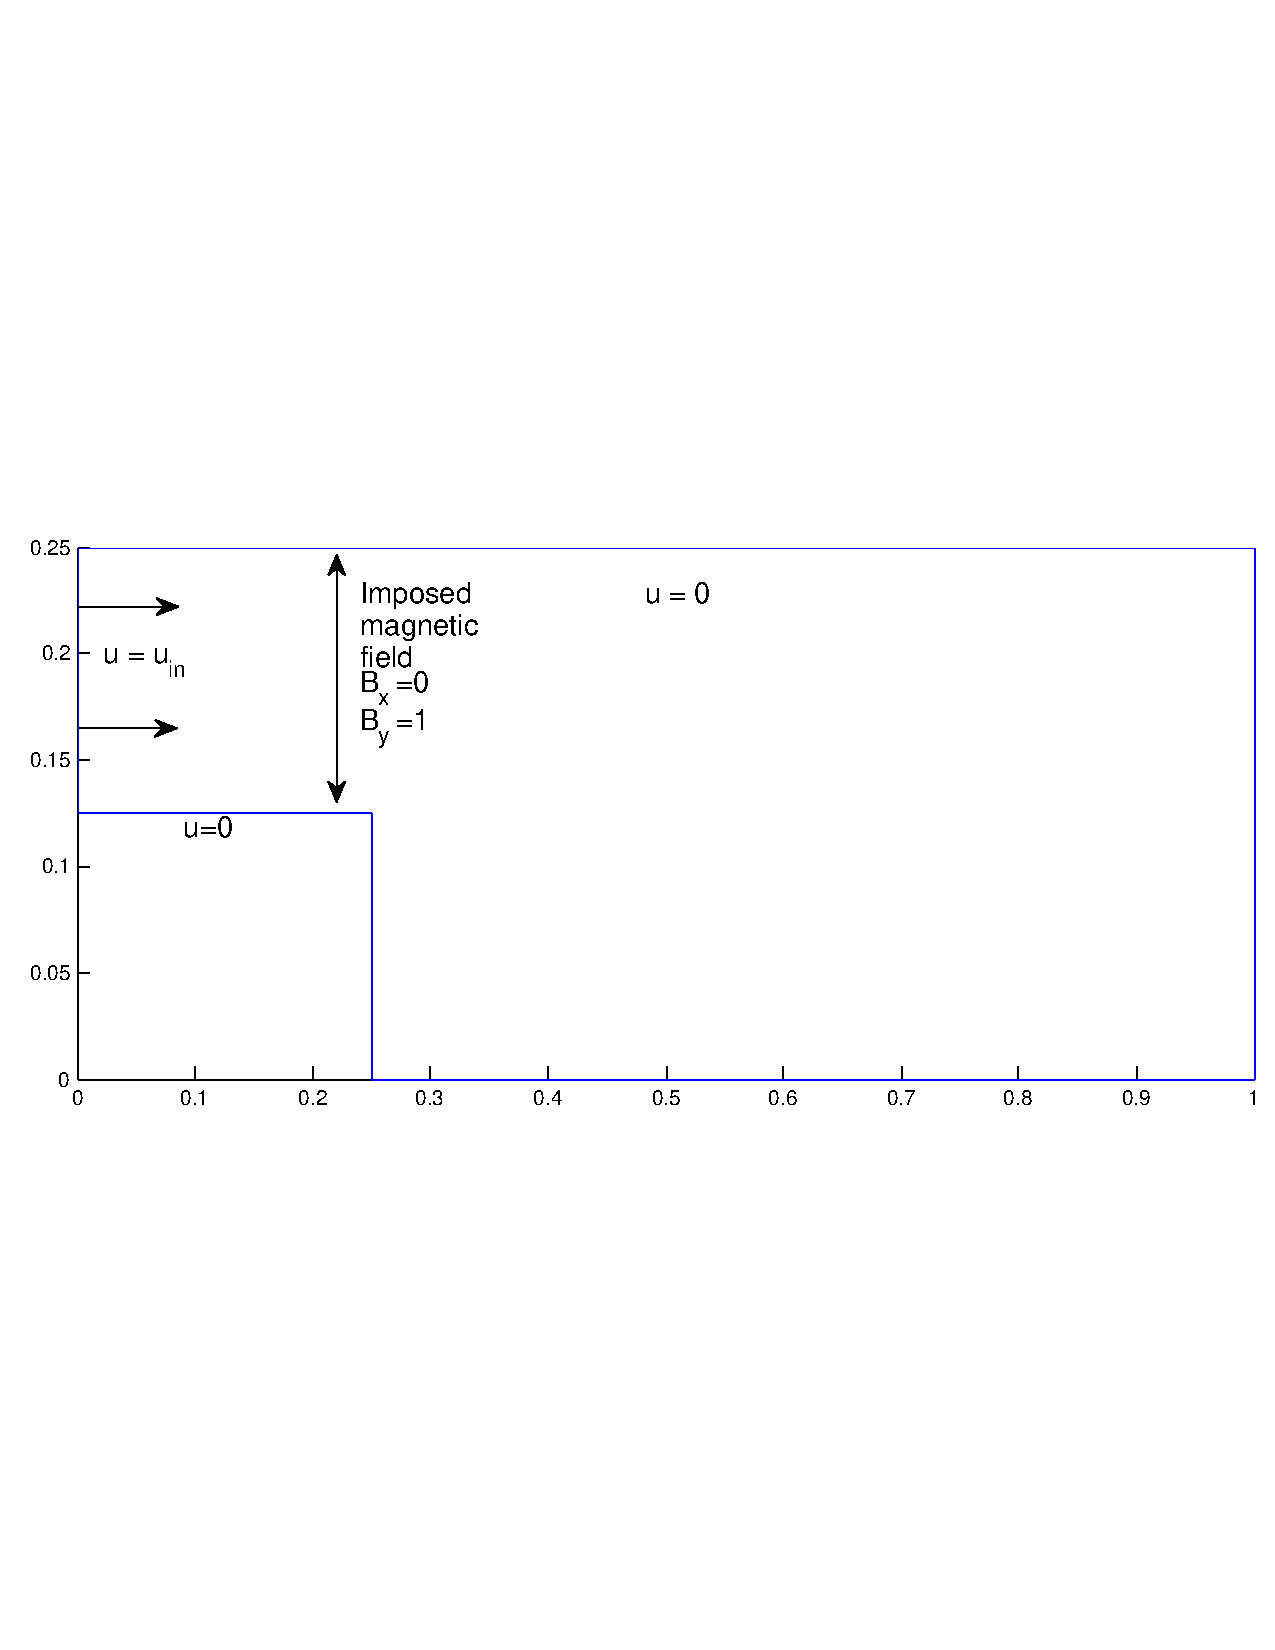
\includegraphics[width=1\textwidth,height=0.3\textwidth, viewport=0 250 640 550, clip]{Domain.pdf}
\caption{\label{stepdomain} The domain and boundary conditions for the MHD channel flow simulation.}
\end{center}
\end{figure}

We compute a DNS for the flow up to $T=10$, using $\alpha_1=\alpha_2=0$ and a mesh that provides 102,650 degrees of freedom and a timestep of $\Delta t=0.01$.  A plot of the velocity field is shown in Figure \ref{mhdchannel_dnsfine}, and this agrees with the expected physical behavior \cite{CS06,Gerbeau00,W12}.

\begin{figure}[htb]
\begin{center}
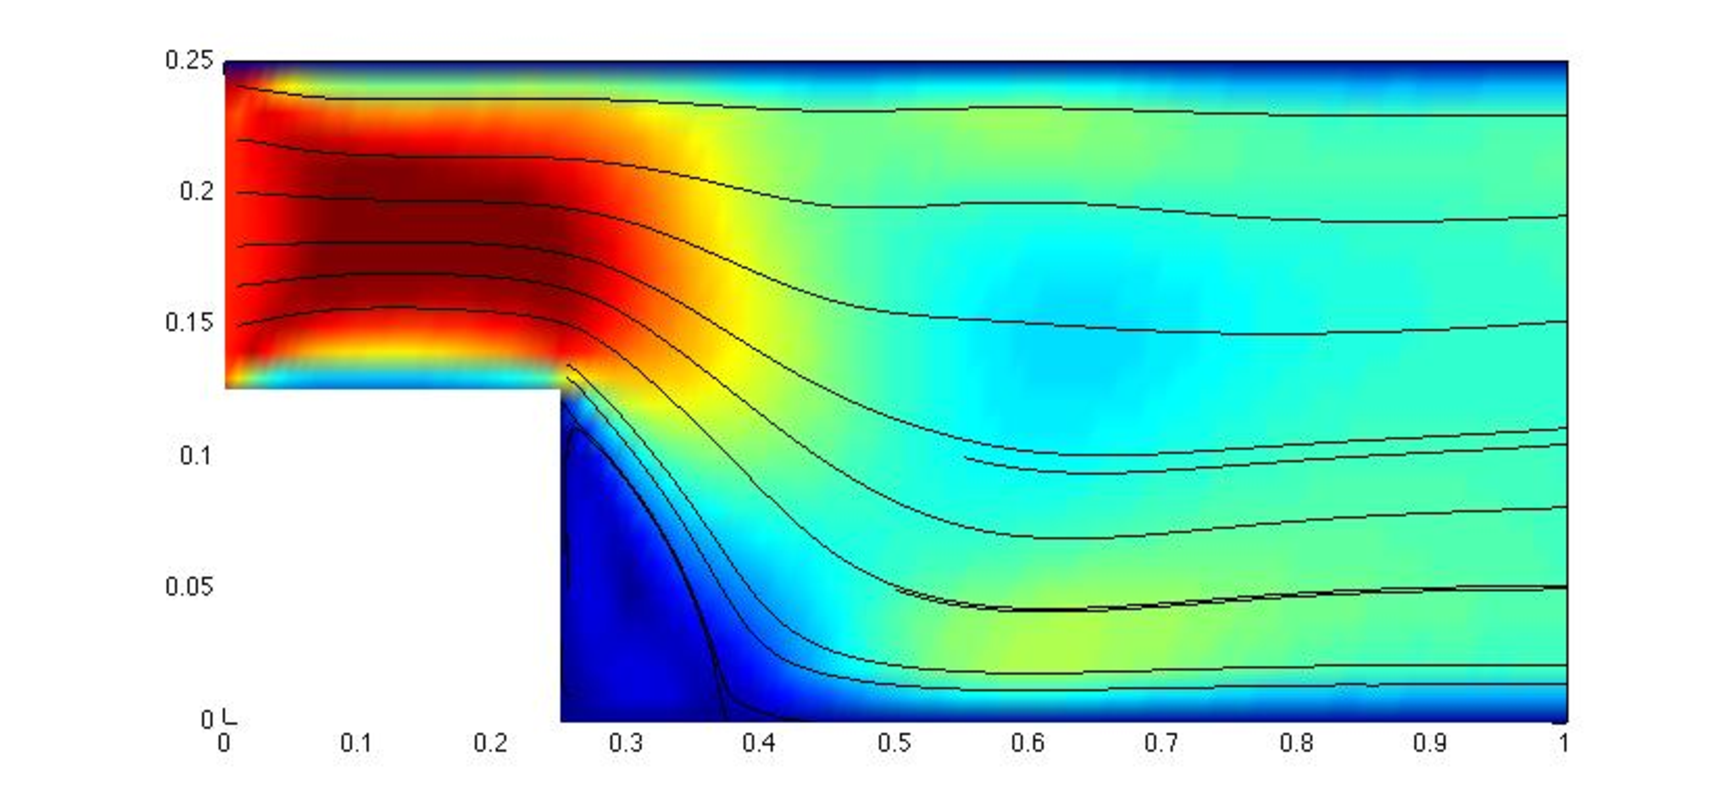
\includegraphics[width=.9\textwidth,height=0.25\textwidth, viewport=110 50 780 370, clip]{MHDChannel_DNSfine.pdf}
\caption{\label{mhdchannel_dnsfine} The velocity field as streamlines over speed contours for the resolved MHD channel flow solution, found using a fine mesh and DNS $\alpha_1=\alpha_2=0$.}
\end{center}
\end{figure}

We also compute on a much coarser discretization, as it is the goal of a fluid flow model to get an accurate (in some sense) answer on a coarse mesh than is needed by a DNS.  Hence we used a mesh that provided 8,666 degrees of freedom and a timestep of $\Delta t=0.1$.  The velocity solution of the DNS $(\alpha_1=\alpha_2=0)$ is shown in Figure \ref{mhdchannel_dnscoarse}, and oscillations are clearly visible in the solution.  The Voigt regularization, on the other hand,
with $\alpha_1=\alpha_2=0.05$ is able to give a smooth and qualitatively accurate solution, on this coarse discretization.

\begin{figure}[htb]
\begin{center}
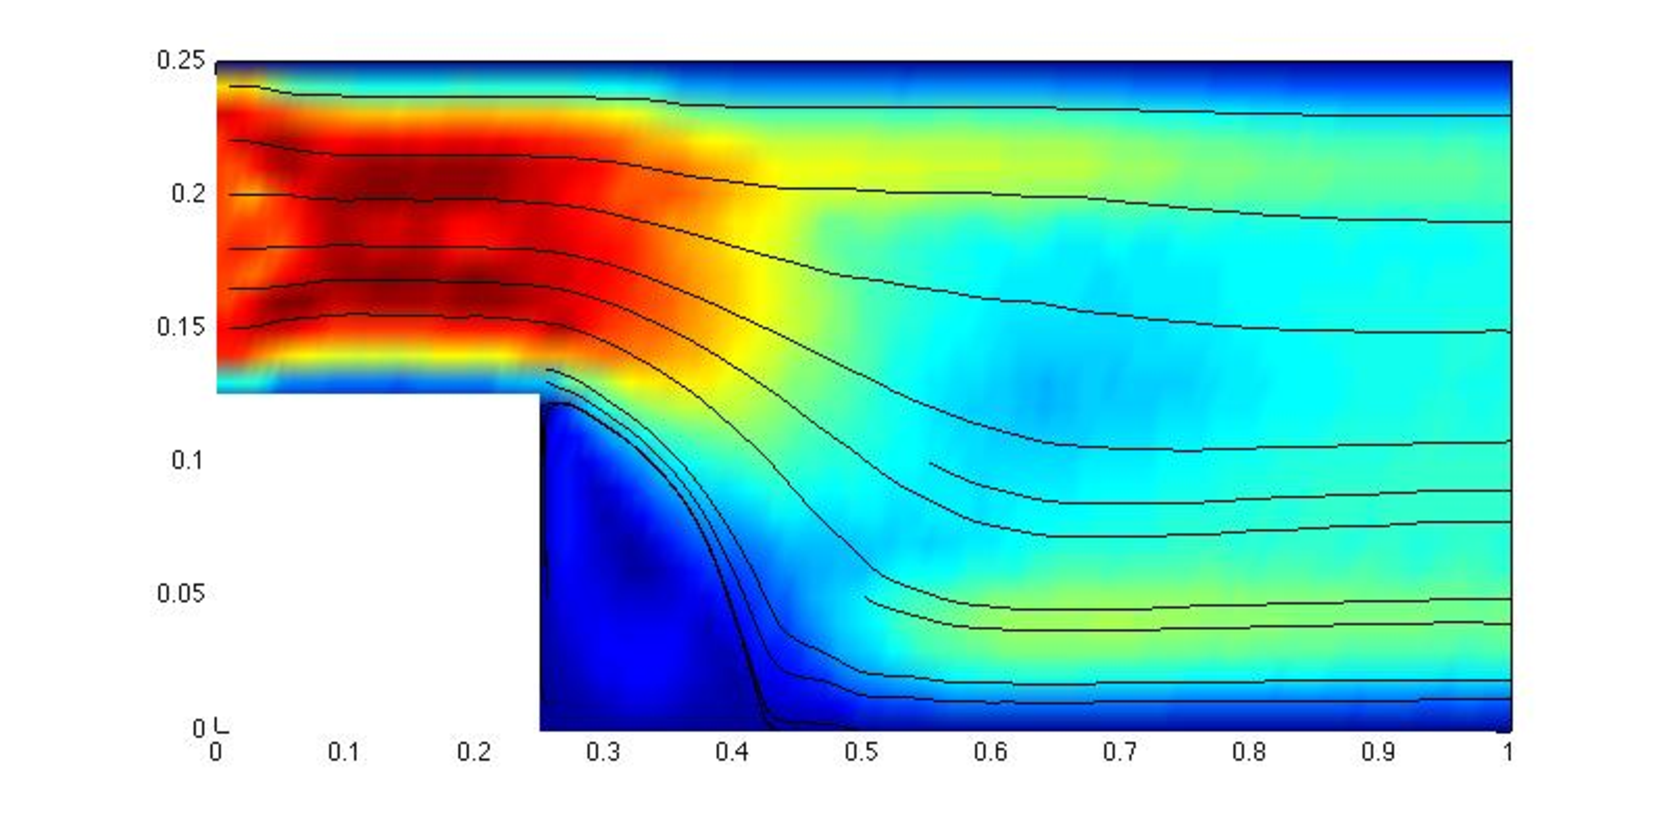
\includegraphics[width=.9\textwidth,height=0.25\textwidth, viewport=110 50 750 370, clip]{MHDChannel_DNScoarse.pdf}
\caption{\label{mhdchannel_dnscoarse} The velocity solution as streamlines over speed contours, found using a DNS  ($\alpha_1=\alpha_2=0$) on a coarse mesh.}
\end{center}
\end{figure}

\begin{figure}[htb]
\begin{center}
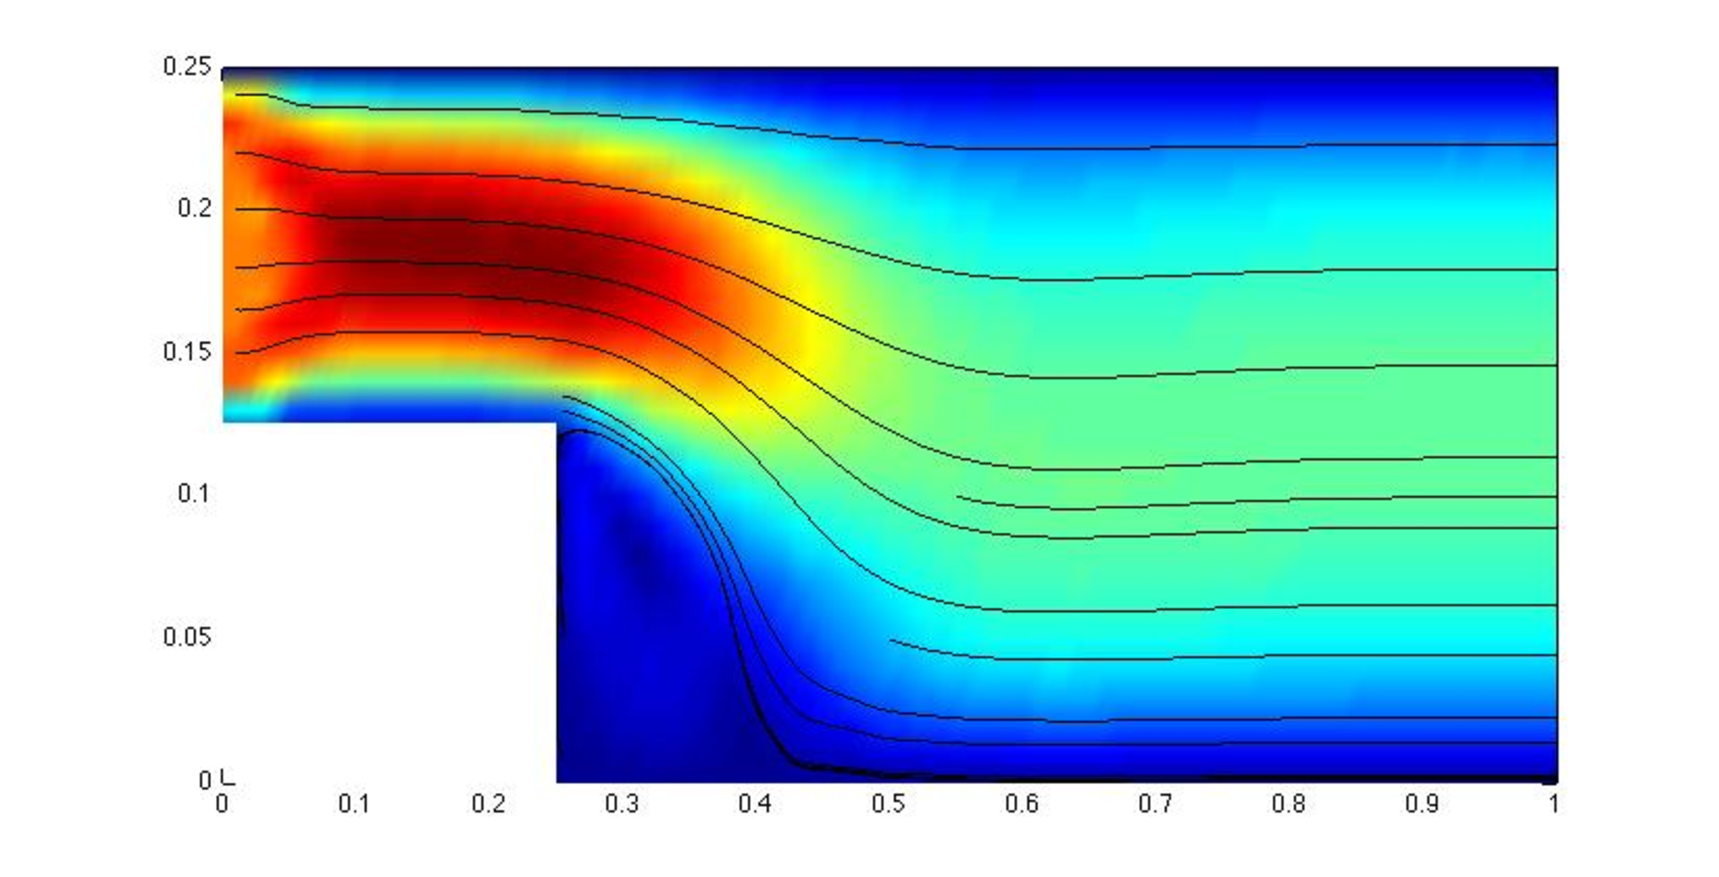
\includegraphics[width=.9\textwidth,height=0.25\textwidth, viewport=110 50 750 370, clip]{MHDChannel_VoigtCoarse.pdf}
\caption{\label{mhdchannel_voigtcoarse} The velocity solution as streamlines over speed contours, found using the Voigt regularization  ($\alpha_1=0.05, \ \alpha_2=0.05$) on a coarse mesh.}
\end{center}
\end{figure}




\subsubsection{Orszag-Tang vortex}

For our final experiment, we repeat a calculation done by J.-G Liu and W. Wang in \cite{LW04}, Friedel et. al. in \cite{FGM97}, and the authors in \cite{CLRW10}, known as the incompressible Orszag-Tang vortex problem for MHD.  This test problem
is for ideal 2D MHD, with $Re=Re_m=\infty$, ${f}=\nabla \times {g}= { 0}$, $s=1$, and compute on the $2\pi$ periodic box with initial condition
\[
u_0 = <-\sin(y+2),\sin(x+1.4)>^T \ \ \ \ \ B_0=<-\frac13 \sin(y+6.2),\frac23 \sin(2x+2.3) >^T
\]
The solution is known to develop singularity-like structures known as current sheets, where
the current density grows exponentially in time, and the thickness of the sheet shrinks at an exponential rate.  By T=2.7, the formation of the sheets is known to occur, and can be seen in the contour plot of $ \nabla \times B $ (which is a scalar in 2D).

We compute with the scheme \eqref{Crank1}-\eqref{Crank4} using $(X_h,Q_h)=(P_3,P_2^{disc})$ Scott-Vogelius elements on a barycenter refinement of a uniform triangulation of $(-\pi,\pi)^2$.  It was shown in \cite{CLRW10} that this choice of mixed finite element is a good choice for such a scheme, as it enforces that both the discrete velocity and magnetic field will satisfy the incompressibility constraint pointwise.

We first compute a reference solution on a fine mesh that provides 345,092 total degrees of freedom, with a timestep of 
 $\Delta t=0.01$ timesteps were used up to $T=2.7$.  The plot of the current density at $T=2.7$ for this solution is shown in Figure \ref{orszag}.  This solution agrees well with the results in \cite{LW04,FGM97,CLRW10}.

\begin{figure}[htb]
\begin{center}
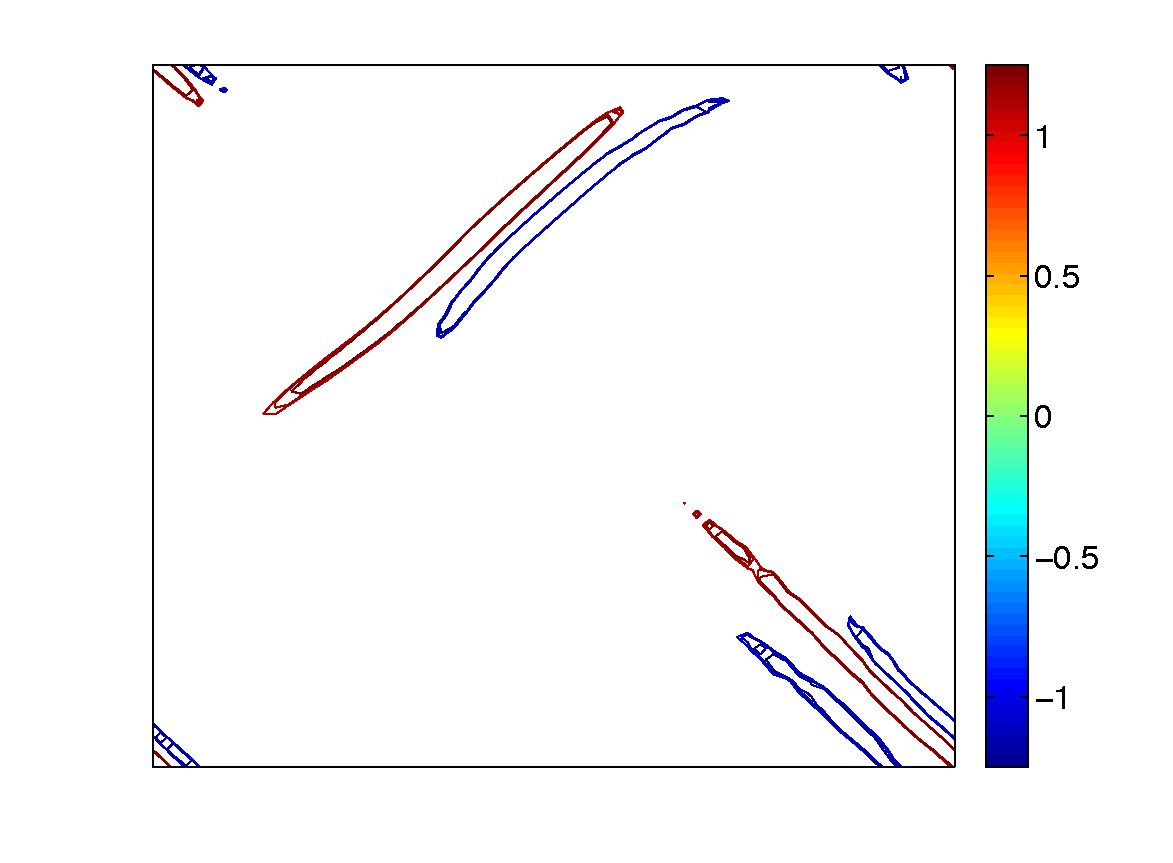
\includegraphics[width=.5\textwidth,height=0.5\textwidth, viewport=70 20 530 400, clip]{MHD_TO_DNS_fine.pdf}
\caption{\label{orszag} The current density of the fine mesh solution $\nabla \times B$ at $T=2.7$.}
\end{center}
\end{figure}

On the coarse mesh, we computed both MHD-Voigt and usual MHD ($\alpha_1=\alpha_2=0$, for comparison.  This mesh provided only 15,748 dof, and we also used a larger timestep, $\Delta t=0.1$.  Hence these coarse mesh computations run in several minutes, while the fine mesh computations take several hours.  For MHD-Voigt, we took $\alpha_1=0.1 \approx h$, and we took $\alpha_2=0$; we found for this problem, any regularization of the magnetic field appears to prohibit the formation of current sheets.  Still, as can be seen in the results in Figure \ref{orszagcoarse}, Voigt regularization of just the velocity provides a good coarse mesh approximation to the true soluion.  The usual MHD run on the coarse mesh is observed to be underresolved.

\begin{figure}[htb]
\begin{center}
\ \ \ \ MHD ($\alpha_1=\alpha_2=0$) \ \ \ \ \ \ \ \ \ \ \ \ \ \ \ \ \ \ MHD-Voigt ($\alpha_1=0.1$, $\alpha_2=0$)
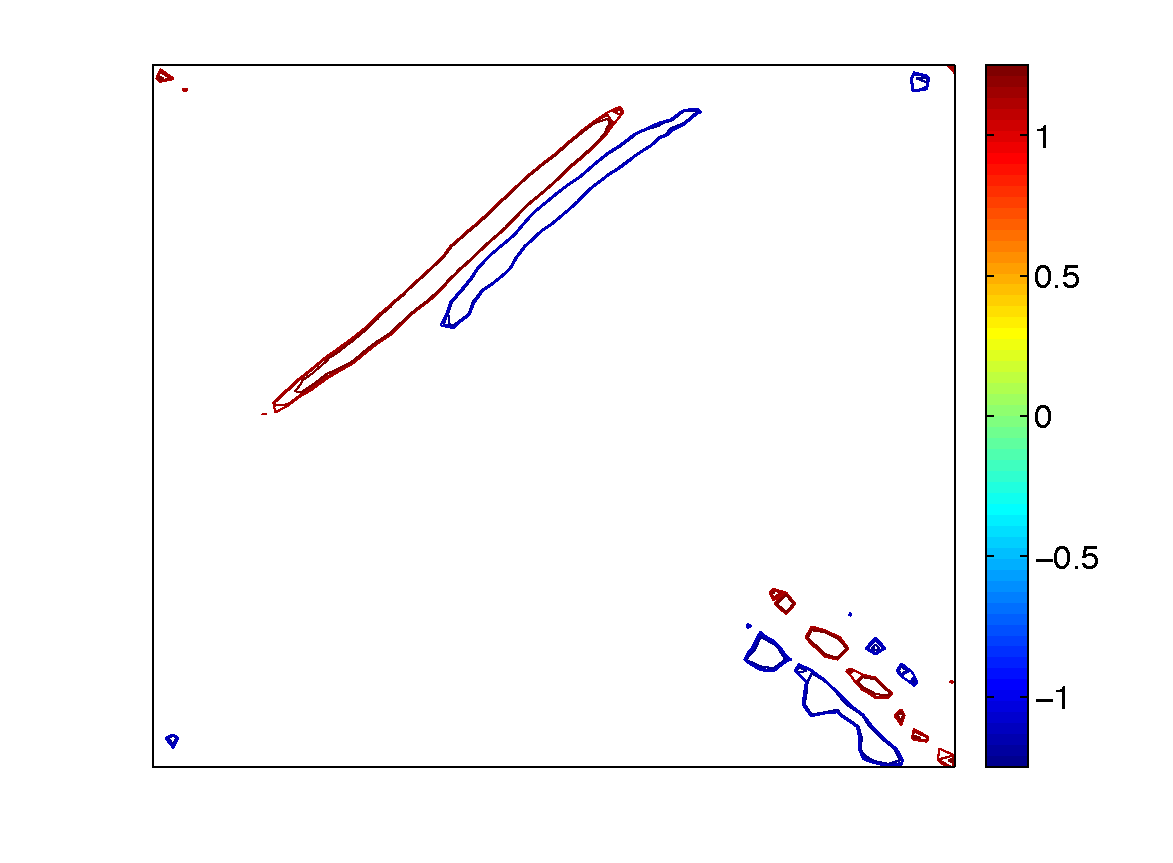
\includegraphics[width=.4\textwidth,height=0.4\textwidth, viewport=70 20 530 400, clip]{MHD_TO_DNS_coarse.pdf}\ \ \ 
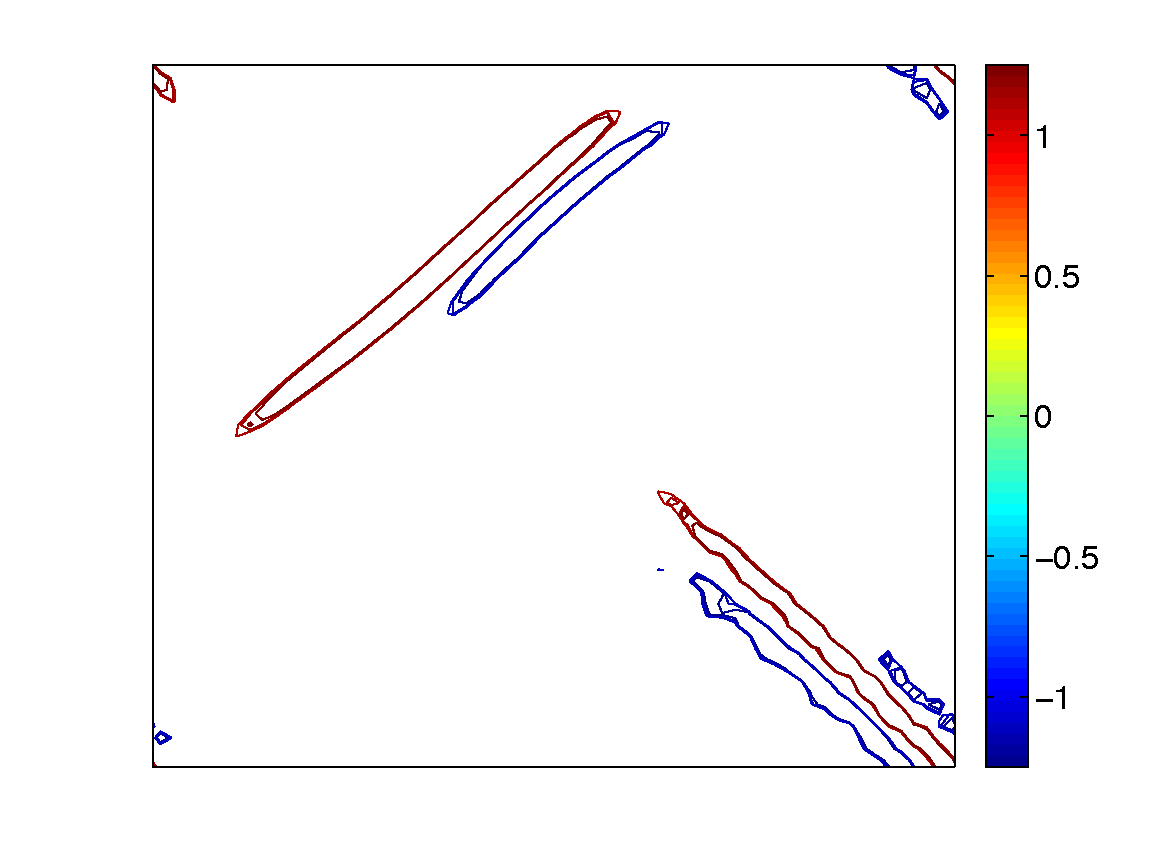
\includegraphics[width=.4\textwidth,height=0.4\textwidth, viewport=70 20 530 400, clip]{MHD_TO_Voigt_coarse.pdf}
\caption{\label{orszagcoarse} The current density of the coarse mesh solutions $\nabla \times B$ at $T=2.7$ for (left) MHD without regularization, and (right) MHD with Voigt regularization of the velocity equation only.}
\end{center}
\end{figure}

{\bf Leo says: We have pics of $\alpha_2>0$ and decreasing to 0 that show that large $\alpha_2$ is bad, but solutions get better as it gets to 0, where it is best.  We are still cleaning up the plots, and will add them in in the near future.}


\section{Conclusion}
This will be the conclusions.

\bibliography{bibliography,LariosBiblio}

\end{document}
